\documentclass[10pt,seperate,ans]{FreshSolution}
\usepackage{minted}
\usepackage{fontspec}
\usepackage{graphicx}
\usepackage{tcolorbox}
\tcbuselibrary{skins, minted}
\renewcommand{\familydefault}{\ttdefault}
\setmonofont{Consolas}
\setminted{
    linenos,
    fontsize=\footnotesize,
    frame=single,
    framesep=2mm,
    numbersep=5pt,
    xleftmargin=10pt,
    breaklines=true,
    tabsize=4,
    showspaces=false,
    showtabs=false,
}
\newtcblisting{codebox}[1][代码]{
  listing engine=minted,         % 使用 minted 引擎
  minted language=cpp,           % 默认语言为 cpp,可通过参数指定
  minted options={               % minted 的高亮选项
    fontsize=\small,
    linenos,                     % 显示行号
    breaklines,                  % 自动换行
    autogobble,                  % 自动去除代码缩进
    escapeinside=||,
    bgcolor=white,
    frame=none
  },
  colback=white,          % 背景颜色
  colframe=black!60!white,        % 边框颜色
  listing only,                  % 只显示代码,不显示输出
  arc=0mm,
  title=#1,                % 标题
}



\begin{document}
\begin{spacing}{1.75}
% \tableofcontents
\section{AIModule}
\subsection{接口类}
\begin{codebox}[公共成员函数]
AIModule()
virtual void onEnd (bool isWinner)
virtual void onFrame ()
virtual void onNukeDetect(Position target)
virtual void onPlayerLeft(Player player)
virtual void onReceiveText(Player player, std::string text)
virtual void onSaveGame(std::string gameName)
virtual void onSendText(std::string text)
virtual void onStart()
virtual void onUnitComplete(Unit unit)
virtual void onUnitCreate(Unit unit)
virtual void onUnitDestroy(Unit unit)
virtual void onUnitDiscover(Unit unit)
virtual void onUnitEvade(Unit unit)
virtual void onUnitHide(Unit unit)
virtual void onUnitMorph(Unit unit)
virtual void onUnitRenegade(Unit unit)
virtual void onUnitShow(Unit unit)
\end{codebox}

\subsubsection{详细描述}
AIModule是一个虚拟类,旨在由自定义AI类实现或继承。

如果BWAPI调用了任何这些预定义的接口功能,则保证初始化Broodwar接口

\begin{warning}
    在调用这些函数的线程以外的任何线程中使用BWAPI都会产生意外行为,并可能崩溃您的Bot。只要所有BWAPI交互都仅限于调用线程,多线程AI是有可能实现的。
    
\end{warning}

\begin{note}
    replay被认为是game,并调用与标准game相同的所有callbacks。
\end{note}
\subsubsection{构造函数和析构函数文档}
\begin{codebox}[构造函数\&析构函数]
    BWAPI::AIModule::AIModule ()
\end{codebox}
\subsubsection{成员函数文档}
\begin{tcolorbox}[colback=white, colframe=black!60!white, title=onStart(), arc=0mm]
    \begin{minted}[frame=none]{cpp}
    virtual void BWAPI::AIModule::onStart()
    \end{minted}
    此函数仅在游戏开始时调用一次。  
    它旨在让 AI 模块在此函数中进行任何数据初始化。
    \begin{warning}
        在调用此函数之前使用 Broodwar 接口可能会导致未定义行为,并使你的 AIbot 崩溃。(例如,在类的静态初始化期间调用接口可能会导致问题。)
    \end{warning}
\end{tcolorbox}
    
\begin{tcolorbox}[colback=white, colframe=black!60!white, title=onEnd(), arc=0mm]
\begin{minted}[frame=none]{cpp}
virtual void BWAPI::AIModule::onEnd(bool isWinner)
\end{minted}
只在游戏结束时被调用一次。
\begin{parameter}
    \begin{itemize}
        \item \texttt{isWinner}:决定当前 player 是否赢得本场比赛的 bool 变量,在获胜时值为 true,在失败或游戏是 replay 时值为 false
    \end{itemize}
\end{parameter}
\end{tcolorbox}

\begin{tcolorbox}[colback=white, colframe=black!60!white, title=onFrame(), arc=0mm]
    \begin{minted}[frame=none]{cpp}
    virtual void BWAPI::AIModule::onFrame()
    \end{minted}
    在每个逻辑帧中被调用一次。  
    用户将大部分代码放在这个函数中。
\end{tcolorbox}
    

\begin{tcolorbox}[colback=white, colframe=black!60!white, title=onSendText(), arc=0mm]
\begin{minted}[frame=none]{cpp}
virtual void BWAPI::AIModule::onSendText(std::string text)
\end{minted}
在 user 尝试发送消息时被调用。  
这个函数让 bot 能够执行 user 输入的文本指令用以 debug。
\begin{parameter}
    \begin{itemize}
        \item \texttt{text}:String 对象,包含 user 发送的具体文本信息
    \end{itemize}
\end{parameter}
\begin{note}
    如果 Flag::UserInput 被禁用,该函数不会被调用。
\end{note}
\end{tcolorbox}

\begin{tcolorbox}[colback=white, colframe=black!60!white, title=onReceiveText(), arc=0mm]
    \begin{minted}[frame=none]{cpp}
    virtual void BWAPI::AIModule::onReceiveText(Player player, std::string text)
    \end{minted}
    在 client 接收到来自另一位 player 的消息时被调用。  
    该函数能用于在团队游戏中从队友处检索信息,或只是为了回应其他 player。
    \begin{parameter}
        \begin{itemize}
            \item \texttt{player}:Player 接口对象代表文本消息的所有者
            \item \texttt{text}:player 发送的文本信息
        \end{itemize}
    \end{parameter}
    \begin{note}
        当前 player 发送的信息不会调用此函数。
    \end{note}
\end{tcolorbox}
    
\begin{tcolorbox}[colback=white, colframe=black!60!white, title=onPlayerLeft(), arc=0mm]
\begin{minted}[frame=none]{cpp}
virtual void BWAPI::AIModule::onPlayerLeft(Player player)
\end{minted}
当一个 player 离开时被调用。  
他们的所有 unit 将会自动分配给 neutral player,并保留他们的 colour 和 alliance 参数。
\begin{parameter}
    \begin{itemize}
        \item \texttt{player}:表示离开游戏的 player 的 Player 接口对象
    \end{itemize}
\end{parameter}
\end{tcolorbox}

\begin{tcolorbox}[colback=white, colframe=black!60!white, title=onNukeDetect(), arc=0mm]
    \begin{minted}[frame=none]{cpp}
    virtual void BWAPI::AIModule::onNukeDetect(Position target)
    \end{minted}
    当 Nuke 在地图上的某个位置启动时调用。
    \begin{parameter}
        \begin{itemize}
            \item \texttt{target}:包含 Nuke 目标位置的 Position 对象。如果目标位置不可见且 Flag::CompleteInformation 已禁用,则目标将为 Position::Unknown
        \end{itemize}
    \end{parameter}
\end{tcolorbox}
    
\begin{tcolorbox}[colback=white, colframe=black!60!white, title=onUnitDiscover(), arc=0mm]
\begin{minted}[frame=none]{cpp}
virtual void BWAPI::AIModule::onUnitDiscover(Unit unit)
\end{minted}
当一个 Unit 变为可访问时调用。
\begin{parameter}
    \begin{itemize}
        \item \texttt{unit}:Unit 接口对象,表示刚刚变为可访问的 unit
    \end{itemize}
\end{parameter}
\begin{note}
    此函数包含 Flag::CompleteMapInformation 状态
\end{note}
\begin{refer}
    \begin{itemize}
        \item \texttt{BWAPI::AIModule::onUnitShow}
    \end{itemize}
\end{refer}
\end{tcolorbox}

\begin{tcolorbox}[colback=white, colframe=black!60!white, title=onUnitEvade(), arc=0mm]
    \begin{minted}[frame=none]{cpp}
    virtual void BWAPI::AIModule::onUnitEvade(Unit unit)
    \end{minted}
    当一个 Unit 变为不可访问时调用。
    \begin{parameter}
        \begin{itemize}
            \item \texttt{unit}:Unit 接口对象,表示刚刚变为不可访问的 unit
        \end{itemize}
    \end{parameter}
    \begin{note}
        此函数包含 Flag::CompleteMapInformation 状态
    \end{note}
    \begin{refer}
        \begin{itemize}
            \item \texttt{BWAPI::AIModule::onUnitHide}
        \end{itemize}
    \end{refer}
\end{tcolorbox}
    
\begin{tcolorbox}[colback=white, colframe=black!60!white, title=onUnitShow(), arc=0mm]
\begin{minted}[frame=none]{cpp}
virtual void BWAPI::AIModule::onUnitShow(Unit unit)
\end{minted}
当以前不可见的 Unit 变为可见时调用。
\begin{parameter}
    \begin{itemize}
        \item \texttt{unit}:Unit 接口对象,表示刚刚变为可见的 unit
    \end{itemize}
\end{parameter}
\begin{note}
    此函数包含 Flag::CompleteMapInformation 状态
\end{note}
\begin{refer}
    \begin{itemize}
        \item \texttt{BWAPI::AIModule::onUnitDiscover}
    \end{itemize}
\end{refer}
\end{tcolorbox}

\begin{tcolorbox}[colback=white, colframe=black!60!white, title=onUnitHide(), arc=0mm]
\begin{minted}[frame=none]{cpp}
virtual void BWAPI::AIModule::onUnitHide(Unit unit)
\end{minted}
当以前可见的 Unit 变为不可见时调用。
\begin{parameter}
    \begin{itemize}
        \item \texttt{unit}:Unit 接口对象,表示即将超出范围的 unit
    \end{itemize}
\end{parameter}
\begin{note}
    此函数包含 Flag::CompleteMapInformation 状态
\end{note}
\begin{refer}
    \begin{itemize}
        \item \texttt{BWAPI::AIModule::onUnitEvade}
    \end{itemize}
\end{refer}
\end{tcolorbox}
\begin{tcolorbox}[colback=white, colframe=black!60!white, title=onUnitCreate(), arc=0mm]
    \begin{minted}[frame=none]{cpp}
    virtual void BWAPI::AIModule::onUnitCreate(Unit unit)
    \end{minted}
    在创建任何 unit 时调用。
    \begin{parameter}
        \begin{itemize}
            \item \texttt{unit}:Unit 接口对象,表示刚刚创建的 unit
        \end{itemize}
    \end{parameter}
    \begin{note}
        由于 Broodwar 的内部机制,此函数排除了 Zerg 的变形(morphing)以及在瓦斯矿(Vespene Geyser)上建造建筑的情况。
    \end{note}
    \begin{refer}
        \begin{itemize}
            \item \texttt{BWAPI::AIModule::onUnitMorph}
        \end{itemize}
    \end{refer}
\end{tcolorbox}

\begin{tcolorbox}[colback=white, colframe=black!60!white, title=onUnitDestroy(), arc=0mm]
\begin{minted}[frame=none]{cpp}
virtual void BWAPI::AIModule::onUnitDestroy(Unit unit)
\end{minted}
当一个 unit 因死亡或其他原因从游戏中移除时被调用。
\begin{parameter}
    \begin{itemize}
        \item \texttt{unit}:Unit 接口对象,表示刚刚被摧毁或以其他方式完全从游戏中移除的 unit
    \end{itemize}
\end{parameter}
\begin{note}
    当一个工蜂(Drone)变形为萃取器(Extractor)时,工蜂会被从游戏中移除,而瓦斯矿(Vespene Geyser)会变形为萃取器。  
    如果一个 unit 是可见的,并且被摧毁,那么在调用此事件之前,会先调用 \texttt{onUnitHide}。
\end{note}
\end{tcolorbox}

\begin{tcolorbox}[colback=white, colframe=black!60!white, title=onUnitMorph(), arc=0mm]
    \begin{minted}[frame=none]{cpp}
    virtual void BWAPI::AIModule::onUnitMorph(Unit unit)
    \end{minted}
    当一个 unit 的 UnitType 发生变化时被调用。  
    例如,当一个工蜂(Drone)变形为孵化场(Hatchery)、攻城坦克(Siege Tank)进入攻城模式(Siege Mode),或者一个瓦斯矿(Vespene Geyser)被建造了精炼厂(Refinery)时。
    \begin{parameter}
        \begin{itemize}
            \item \texttt{unit}:Unit 接口对象,表示 UnitType 的改变的 unit
        \end{itemize}
    \end{parameter}
    \begin{note}
        如果 UnitType 变为或从 \texttt{UnitTypes::Unknown} 变化,则不会触发此事件。
    \end{note}
\end{tcolorbox}
    
\begin{tcolorbox}[colback=white, colframe=black!60!white, title=onUnitRenegade(), arc=0mm]
\begin{minted}[frame=none]{cpp}
virtual void BWAPI::AIModule::onUnitRenegade(Unit unit)
\end{minted}
当一个 unit 的所有权发生变化时被调用。  
这种情况发生在使用神族的“心灵控制”(Mind Control)技能时,或者在“使用地图设置”(Use Map Settings)中单位的所有权发生变化时。
\begin{parameter}
    \begin{itemize}
        \item \texttt{unit}:Unit 接口对象,表示改变所有权的 unit
    \end{itemize}
\end{parameter}
\end{tcolorbox}
\begin{tcolorbox}[colback=white, colframe=black!60!white, title=onSaveGame(), arc=0mm]
    \begin{minted}[frame=none]{cpp}
    virtual void BWAPI::AIModule::onSaveGame(std::string gameName)
    \end{minted}
    当 Broodwar 游戏状态被保存到文件时被调用。
    \begin{parameter}
        \begin{itemize}
            \item \texttt{gameName}:包含游戏被保存为的文件名的 String 对象
        \end{itemize}
    \end{parameter}
\end{tcolorbox}

\begin{tcolorbox}[colback=white, colframe=black!60!white, title=onUnitComplete(), arc=0mm]
\begin{minted}[frame=none]{cpp}
virtual void BWAPI::AIModule::onUnitComplete(Unit unit)
\end{minted}
当 unit 的状态从 'incomplete' 变为 'complete' 时被调用。
\begin{parameter}
    \begin{itemize}
        \item \texttt{unit}:Unit 对象,表示刚刚完成训练或建造的 Unit
    \end{itemize}
\end{parameter}
\end{tcolorbox}

% \tableofcontents
\section{BulletInterface}
\subsection{接口类}
\subsection{BWAPI::BulletInterface继承图}
\begin{figure}[H]
    \centering
    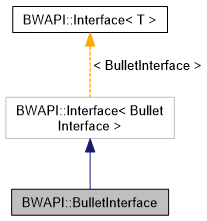
\includegraphics[width=0.4\textwidth]{figures/BulletInterface继承图.png}
\end{figure}
\subsubsection{公共成员函数}
\begin{codebox}[公共成员函数]
virtual bool exists () const =0
virtual double getAngle () const =0
virtual int getID () const =0
virtual Player getPlayer () const =0
virtual Position getPosition () const =0
virtual int getRemoveTimer () const =0
virtual Unit getSource () const =0
virtual Unit getTarget () const =0
virtual Position getTargetPosition () const =0
virtual BulletType getType () const =0
virtual double getVelocityX () const =0
virtual double getVelocityY () const =0
virtual bool isVisible (Player player=nullptr) const =0
\end{codebox}
\subsubsection{详细描述}
接口对象,表示从攻击中生成的子弹或飞弹。\par
Bullet 接口允许你检测子弹、飞弹以及其他类型的非近战攻击或特殊能力,这些通常是人类玩家通过视觉可以看到的(例如潜伏者的地刺或女皇的寄生飞虫)。这使得 AI 可以更快地对不可避免的后果做出反应。\par
例如,你可以命令medic提前治疗即将被锁定的unit,以补偿延迟并尽量减少其影响。除非你能够通过 Bullet 类检测到锁定飞弹,否则你无法完全知道哪个unit将被锁定。\par
Bullet 对象在被销毁后会被重新使用,但当它代表一个新的 Bullet 时,其 ID 会被更新。\par
如果禁用了   Flag::CompleteMapInformation  ,那么只有可见的 Bullet 才能被访问。否则,如果启用了   Flag::CompleteMapInformation  ,那么游戏中所有的 Bullet 都可以被访问。\par
\begin{refer}
    \begin{itemize}
        \item Game::getBullets
        \item BulletInterface::exists
    \end{itemize}
\end{refer}

\subsubsection{成员函数文档}

\begin{tcolorbox}[colback=white, colframe=black!60!white, title=getID(), arc=0mm]
\begin{minted}[frame=none]{cpp}
virtual int BWAPI::BulletInterface::getID() const
\end{minted}
获取当前子弹的唯一标识符。
\begin{return}
    \begin{itemize}
            \item int:子弹标识符
    \end{itemize}
\end{return}
\end{tcolorbox}

\begin{tcolorbox}[colback=white, colframe=black!60!white, title=exists(), arc=0mm]
\begin{minted}[frame=none]{cpp}    
virtual bool BWAPI::BulletInterface::exists() const
\end{minted}
检查Bullet是否存在于BWAPI player的视野中。
\begin{return}
    \begin{itemize}
        \item \texttt{bool}:子弹存在或可见(true) / 已被销毁或超出作用范围(false)
    \end{itemize}
\end{return}
如果禁用了  Flag::CompleteMapInformation  ,并且一个  Bullet  不可见,那么无论该bullet是否真实存在,返回值都将为  false  。这是因为对于不可见的敌方bullet,AI无法获取任何状态信息。\par
如果启用了  Flag::CompleteMapInformation  ,那么这个函数对于所有  Bullet  信息都是准确的。
\begin{refer}
    \begin{itemize}
        \item isVisible
        \item UnitInterface::exists
    \end{itemize}
\end{refer}
\end{tcolorbox}

\begin{tcolorbox}[colback=white, colframe=black!60!white, title=getPlayer(), arc=0mm]
    \begin{minted}[frame=none]{cpp}
virtual Player BWAPI::BulletInterface::getPlayer() const
    \end{minted}
    获取拥有该Bullet的Player接口对象。
    \begin{return}
        \begin{itemize}
            \item \texttt{Player}:拥有该Bullet的Player接口对象 / 无法访问该Bullet的Player对象(nullptr)
        \end{itemize}
    \end{return}
\end{tcolorbox}


\begin{tcolorbox}[colback=white, colframe=black!60!white, title=getType(), arc=0mm]
    \begin{minted}[frame=none]{cpp}
virtual BulletType BWAPI::BulletInterface::getType() const
    \end{minted}
    获取当前Bullet的类型。
    \begin{return}
        \begin{itemize}
            \item \texttt{BulletType}:Bullet类型 / Bullet无法访问 (BulletTypes::Unknown)
        \end{itemize}
    \end{return}
\end{tcolorbox}

\begin{tcolorbox}[colback=white, colframe=black!60!white, title=getSource(), arc=0mm]
    \begin{minted}[frame=none]{cpp}
virtual Unit BWAPI::BulletInterface::getSource() const
    \end{minted}
    获取发射这颗Bullet的Unit接口对象。
    \begin{return}
        \begin{itemize}
            \item \texttt{Unit}:拥有该Bullet的Unit接口对象 / 无法识别或访问发射源 (nullptr)
        \end{itemize}
    \end{return}
    \begin{refer}
        \begin{itemize}
            \item getTarget
        \end{itemize}
    \end{refer}
\end{tcolorbox}

\begin{tcolorbox}[colback=white, colframe=black!60!white, title=getPosition(), arc=0mm]
    \begin{minted}[frame=none]{cpp}
virtual Position BWAPI::BulletInterface::getPosition() const
    \end{minted}
    获取Bullet的当前位置。
    \begin{return}
        \begin{itemize}
            \item \texttt{Position}:子弹当前的位置 / 子弹无法访问 (Positions::Unknown)
        \end{itemize}
    \end{return}
    \begin{refer}
        \begin{itemize}
            \item getTargetPosition
        \end{itemize}
    \end{refer}
\end{tcolorbox}

\begin{tcolorbox}[colback=white, colframe=black!60!white, title=getAngle(), arc=0mm]
    \begin{minted}[frame=none]{cpp}
virtual double BWAPI::BulletInterface::getAngle() const
    \end{minted}
    获取Bullet的朝向方向。如果angle为0,则Bullet朝向为right。
    \begin{return}
        \begin{itemize}
            \item double:Bullet的angle / Bullet无法访问 (0.0)
        \end{itemize}
    \end{return}
    \begin{refer}
        \begin{itemize}
            \item getTargetPosition
        \end{itemize}
    \end{refer}
\end{tcolorbox}

\begin{tcolorbox}[colback=white, colframe=black!60!white, title=getVelocityX(), arc=0mm]
    \begin{minted}[frame=none]{cpp}
virtual double BWAPI::BulletInterface::getVelocityX() const
    \end{minted}
    获取Bullet在X轴方向上的速度分量。
    \begin{return}
        \begin{itemize}
            \item double:Bullet每frame在X轴方向上移动的pixel数 / Bullet无法访问 (0.0)
        \end{itemize}
    \end{return}
    \begin{refer}
        \begin{itemize}
            \item getVelocityY
            \item getAngle
        \end{itemize}
    \end{refer}
\end{tcolorbox}

\begin{tcolorbox}[colback=white, colframe=black!60!white, title=getVelocityY(), arc=0mm]
    \begin{minted}[frame=none]{cpp}
virtual double BWAPI::BulletInterface::getVelocityY() const
    \end{minted}
    获取Bullet在Y轴方向上的速度分量。
    \begin{return}
        \begin{itemize}
            \item double:Bullet每frame在Y轴方向上移动的pixel数 / Bullet无法访问 (0.0)
        \end{itemize}
    \end{return}
    \begin{refer}
        \begin{itemize}
            \item getVelocityX
            \item getAngle
        \end{itemize}
    \end{refer}
\end{tcolorbox}

\begin{tcolorbox}[colback=white, colframe=black!60!white, title=getTarget(), arc=0mm]
    \begin{minted}[frame=none]{cpp}
virtual Unit BWAPI::BulletInterface::getTarget() const
    \end{minted}
    获取Bullet的目标Unit接口对象。
    \begin{return}
        \begin{itemize}
            \item \texttt{Unit}:存在目标Unit / Bullet目标Unit无法访问,或者Bullet的目标是ground,或者Bullet本身无法访问 (nullptr)
        \end{itemize}
    \end{return}
    \begin{refer}
        \begin{itemize}
            \item getTargetPosition
            \item getSource
        \end{itemize}
    \end{refer}
\end{tcolorbox}

\begin{tcolorbox}[colback=white, colframe=black!60!white, title=getTargetPosition(), arc=0mm]
    \begin{minted}[frame=none]{cpp}
virtual Position BWAPI::BulletInterface::getTargetPosition() const
    \end{minted}
    获取Bullet的目标位置。
    \begin{return}
        \begin{itemize}
            \item \texttt{Position}:Bullet的飞行目标位置 / Bullet无法访问 (Positions::Unknown)
        \end{itemize}
    \end{return}
    \begin{refer}
        \begin{itemize}
            \item getTarget
            \item getPosition
        \end{itemize}
    \end{refer}
\end{tcolorbox}

\begin{tcolorbox}[colback=white, colframe=black!60!white, title=getRemoveTimer(), arc=0mm]
    \begin{minted}[frame=none]{cpp}
virtual int BWAPI::BulletInterface::getRemoveTimer() const
    \end{minted}
    获取Bullet的剩余寿命。Bullet不是永久对象,通常有一个有限的寿命,以frame为单位测量。
    \begin{return}
        \begin{itemize}
            \item int:Bullet自毁前剩余的frame数 / Bullet无法访问 (0)
        \end{itemize}
    \end{return}
    \begin{refer}
        \begin{itemize}
            \item getTarget
            \item getPosition
        \end{itemize}
    \end{refer}
\end{tcolorbox}

\begin{tcolorbox}[colback=white, colframe=black!60!white, title=isVisible(), arc=0mm]
    \begin{minted}[frame=none]{cpp}
virtual bool BWAPI::BulletInterface::isVisible(Player player = nullptr) const
    \end{minted}
    获取Bullet的可见性状态。
    \begin{parameter}
        \begin{itemize}
            \item \texttt{player}(可选):如果指定了这个参数,则检查该player是否能看到这颗bullet。如果未指定此参数,则使用默认值nullptr,此时会检查BWAPI player是否能看到这颗bullet。
        \end{itemize}
    \end{parameter}
    \begin{note}
        如果player是nullptr,并且Broodwar->self()也是nullptr,则通过检查是否有其他player能看到这颗bullet来确定其可见性。
    \end{note}
    \begin{return}
        \begin{itemize}
            \item \texttt{bool}:指定player可以看到这颗bullet (true) / 指定player看不到这颗bullet (false)
        \end{itemize}
    \end{return}
\end{tcolorbox}
% \tableofcontents
\section{UnitType}
\subsection{接口类}
\subsection{BWAPI::UnitType继承图}
\begin{figure}[H]
    \centering
    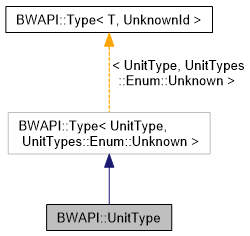
\includegraphics[width=0.4\textwidth]{figures/UnitType继承图.png}
\end{figure}
\subsubsection{公共成员函数}
\begin{codebox}[公共成员函数]
constexpr UnitType (int id=UnitTypes::Enum::None)
const SetContainer< TechType > & abilities () const
int acceleration () const
WeaponType airWeapon () const
int armor () const
UpgradeType armorUpgrade () const
int buildScore () const
const UnitType::set & buildsWhat () const
\end{codebox}
\begin{codebox}[公共成员函数]
int buildTime () const
bool canAttack () const
bool canBuildAddon () const
bool canMove () const
bool canProduce () const
TechType cloakingTech () const
int destroyScore () const
int dimensionDown () const
int dimensionLeft () const
int dimensionRight () const
int dimensionUp () const
int gasPrice () const
Race getRace () const
WeaponType groundWeapon () const
int haltDistance () const
bool hasPermanentCloak () const
int height () const
bool isAddon () const
bool isBeacon () const
bool isBuilding () const
bool isBurrowable () const
bool isCloakable () const
bool isCritter () const
bool isDetector () const
bool isFlagBeacon () const
bool isFlyer () const
bool isFlyingBuilding () const
bool isHero () const
bool isInvincible () const
bool isMechanical () const
bool isMineralField () const
bool isNeutral () const
\end{codebox}
\begin{codebox}[公共成员函数]
bool isOrganic () const
bool isPowerup () const
bool isRefinery () const
bool isResourceContainer () const
bool isResourceDepot () const
bool isRobotic () const
bool isSpecialBuilding () const
bool isSpell () const
bool isSpellcaster () const
bool isSuccessorOf (UnitType type) const
bool isTwoUnitsInOneEgg () const
bool isWorker () const
int maxAirHits () const
int maxEnergy () const
int maxGroundHits () const
int maxHitPoints () const
int maxShields () const
int mineralPrice () const
bool producesCreep () const
bool producesLarva () const
bool regeneratesHP () const
TechType requiredTech () const
const std::map< UnitType, int > & requiredUnits () const
bool requiresCreep () const
bool requiresPsi () const
const SetContainer< TechType > & researchesWhat () const
int seekRange () const
int sightRange () const
UnitSizeType size () const
\end{codebox}
\begin{codebox}[公共成员函数]
int spaceProvided () const
int spaceRequired () const
int supplyProvided () const
int supplyRequired () const
int tileHeight () const
TilePosition tileSize () const
int tileWidth () const
double topSpeed () const
int turnRadius () const
const SetContainer< UpgradeType > & upgrades () const
const SetContainer< UpgradeType > & upgradesWhat () const
const std::pair< UnitType, int > whatBuilds () const
int width () const
\end{codebox}
\subsubsection{详细描述}
UnitType 类用于获取特定unit类型的信息,例如unit的成本(cost)、建造时间(build time)、武器(weapon)、生命值(hit points)、能力(abilities)等。
\begin{refer}
\begin{itemize}
    \item UnitInterface::getType
    \item UnitTypes
\end{itemize}
\end{refer}
\subsubsection{构造函数\&析构函数文档}
\begin{tcolorbox}[colback=white, colframe=black!60!white, title=UnitType(), arc=0mm]
    \begin{minted}[frame=none]{cpp}
constexpr BWAPI::UnitType::UnitType (int id = UnitTypes::Enum::None)
    \end{minted}
预期类型构造函数\par
如果type是无效类型(invalid type),则会变成   Types::Unknown  。如果type的值小于 0 或大于   Types::Unknown  ,则该type无效
\begin{parameter}
\begin{itemize}
    \item id:与该type对应的 ID。它通常是一个整数值,对应于 Broodwar 的内部类型。如果给定的 ID 无效,则会变成   Types::Unknown  。
\end{itemize}
\end{parameter}
\end{tcolorbox}

\subsubsection{成员函数文档}

\begin{tcolorbox}[colback=white, colframe=black!60!white, title=abilities(), arc=0mm]
    \begin{minted}[frame=none]{cpp}
const SetContainer<TechType>& BWAPI::UnitType::abilities () const
    \end{minted}
检索此Unit在游戏中可用的技能集合。
\begin{return}
\begin{itemize}
    \item SetContainer<TechType>:包含技能信息的   TechTypes   集合。
\end{itemize}
\end{return}
\end{tcolorbox}


\begin{tcolorbox}[colback=white, colframe=black!60!white, title=acceleration(), arc=0mm]
    \begin{minted}[frame=none]{cpp}
int BWAPI::UnitType::acceleration () const
    \end{minted}
检索unit的加速度。
\begin{return}
\begin{itemize}
    \item int:unit达到最高速度的加速度。
\end{itemize}
\end{return}
\end{tcolorbox}

\begin{tcolorbox}[colback=white, colframe=black!60!white, title=airWeapon(), arc=0mm]
    \begin{minted}[frame=none]{cpp}
WeaponType BWAPI::UnitType::airWeapon () const
    \end{minted}
检索此UnitType的对空WeaponType。
\begin{return}
\begin{itemize}
    \item WeaponType:此UnitType用于攻击空中目标的Weapontype。
\end{itemize}
\end{return}
\end{tcolorbox}


\begin{tcolorbox}[colback=white, colframe=black!60!white, title=armor(), arc=0mm]
    \begin{minted}[frame=none]{cpp}
int BWAPI::UnitType::armor () const
    \end{minted}
检索该UnitType初始的默认护甲值,不包括任何升级。
\begin{note}
此值可能与Use Map Settings游戏类型中看到的值不一致。
\end{note}
\begin{return}
\begin{itemize}
    \item int:UnitType所拥有的护甲值。
\end{itemize}
\end{return}
\end{tcolorbox}


\begin{tcolorbox}[colback=white, colframe=black!60!white, title=armorUpgrade(), arc=0mm]
    \begin{minted}[frame=none]{cpp}
UpgradeType BWAPI::UnitType::armorUpgrade () const
    \end{minted}
检索用于增加此UnitType护甲的升级类型(UpgradeType)\par
每次升级,此UnitType会获得 +1 的额外护甲。
\begin{return}
\begin{itemize}
    \item UpgradeType:表示增加此UnitType护甲数量的升级类型。
\end{itemize}
\end{return}
\end{tcolorbox}


\begin{tcolorbox}[colback=white, colframe=black!60!white, title=buildScore(), arc=0mm]
    \begin{minted}[frame=none]{cpp}
int BWAPI::UnitType::buildScore () const
    \end{minted}
检索建造此UnitType所获得的分数。\par
此值用于计算游戏结束后的得分屏幕上的分数。
\begin{return}
\begin{itemize}
    \item int:建造此UnitType所获得的分数。
\end{itemize}
\end{return}
\end{tcolorbox}


\begin{tcolorbox}[colback=white, colframe=black!60!white, title=buildsWhat(), arc=0mm]
    \begin{minted}[frame=none]{cpp}
const UnitType::set& BWAPI::UnitType::buildsWhat () const
    \end{minted}
    检索此UnitType能够创建的unit集合。\par
    这包括训练、建造、传送和变形。
\begin{note}
    某些地图有特殊参数,可能会禁用通常可以建造的unit。可以使用   PlayerInterface::isUnitAvailable   来确定某个UnitType是否在当前游戏中对特定player可用。
\end{note}
\begin{return}
\begin{itemize}
    \item UnitType::set:包含此UnitType可以建造的unit。
\end{itemize}
\end{return}
\begin{refer}
\begin{itemize}
    \item PlayerInterface::isUnitAvailable  :用于判断某个UnitType是否对特定player可用。
\end{itemize}
\end{refer}
\end{tcolorbox}


\begin{tcolorbox}[colback=white, colframe=black!60!white, title=buildTime(), arc=0mm]
    \begin{minted}[frame=none]{cpp}
int BWAPI::UnitType::buildTime () const
    \end{minted}
    检索训练、变形或建造该unit所需的默认时间,以frame为单位。
\begin{note}
    此值可能与 Use Map Settings 游戏类型中显示的值不一致。
\end{note}
\begin{return}
\begin{itemize}
    \item int:建造该unit所需的frame数。
\end{itemize}
\end{return}
\begin{refer}
\begin{itemize}
    \item UnitInterface::getRemainingBuildTime  :用于获取unit剩余的建造时间。
\end{itemize}
\end{refer}
\end{tcolorbox}


\begin{tcolorbox}[colback=white, colframe=black!60!white, title=canAttack(), arc=0mm]
    \begin{minted}[frame=none]{cpp}
bool BWAPI::UnitType::canAttack () const
    \end{minted}
    检查该unit是否能够进行攻击。
\begin{note}
    对于只能通过特殊技能造成伤害的unit(例如高阶圣堂武士),此函数将返回   false
\end{note}
\begin{return}
\begin{itemize}
    \item bool:如果该UnitType能够通过标准攻击对其他unit造成伤害,则返回   true  ,否则返回   false
\end{itemize}
\end{return}
\end{tcolorbox}


\begin{tcolorbox}[colback=white, colframe=black!60!white, title=canBuildAddon(), arc=0mm]
    \begin{minted}[frame=none]{cpp}
bool BWAPI::UnitType::canBuildAddon () const
    \end{minted}
    检查该UnitType是否能够建造附加建筑。
\begin{return}
\begin{itemize}
    \item bool:如果该UnitType能够建造附加建筑,则返回   true  ,否则返回   false  。
\end{itemize}
\end{return}
\begin{refer}
\begin{itemize}
    \item isAddon  :用于检查某个UnitType是否能附加建筑。
\end{itemize}
\end{refer}
\end{tcolorbox}


\begin{tcolorbox}[colback=white, colframe=black!60!white, title=canMove(), arc=0mm]
    \begin{minted}[frame=none]{cpp}
bool BWAPI::UnitType::canMove () const
    \end{minted}
    检查该UnitType是否能够移动。
\begin{note}
    建筑物将返回   false  ,包括升起时能够移动的 Terran 可升降建筑。
\end{note}
\begin{return}
\begin{itemize}
    \item bool:如果该unit能够使用移动命令,则返回   true  ,否则返回   false
\end{itemize}
\end{return}
\end{tcolorbox}


\begin{tcolorbox}[colback=white, colframe=black!60!white, title=canProduce(), arc=0mm]
    \begin{minted}[frame=none]{cpp}
bool BWAPI::UnitType::canProduce () const
    \end{minted}
    确定一个单位是否能够生产其他单位。\par
    例如\verb|Terran_Barracks.canProduce()|将返回true,而\verb|Terran_Marine.canProduce()|将返回   false  。
    这同样适用于两种非建筑单位:航空母舰(Carrier)可以生产拦截机(interceptors)和雷兽(Reaver)可以生产甲虫(scarabs)
\begin{return}
\begin{itemize}
    \item bool:如果该unit能够使用移动命令,则返回   true  ,否则返回   false
\end{itemize}
\end{return}
\end{tcolorbox}


\begin{tcolorbox}[colback=white, colframe=black!60!white, title=cloakingTech(), arc=0mm]
    \begin{minted}[frame=none]{cpp}
TechType BWAPI::UnitType::cloakingTech () const
    \end{minted}
    检索与某些unit相关的隐形技术。
\begin{return}
\begin{itemize}
    \item TechType:表示该UnitType使用的隐形技术作为能力。\par
    (TechTypes::None  :如果该UnitType没有主动隐形能力。)
\end{itemize}
\end{return}
\end{tcolorbox}


\begin{tcolorbox}[colback=white, colframe=black!60!white, title=destroyScore(), arc=0mm]
    \begin{minted}[frame=none]{cpp}
int BWAPI::UnitType::destroyScore () const
    \end{minted}
    检索击杀该UnitType所获得的分数。\par
    此值用于计算游戏结束后的得分屏幕上的分数。
\begin{return}
\begin{itemize}
    \item int:击杀该UnitType所获得的分数。
\end{itemize}
\end{return}
\begin{refer}
    \begin{itemize}
        \item buildScore:建造该UnitType所获得的分数。
    \end{itemize}
\end{refer}
\end{tcolorbox}


\begin{tcolorbox}[colback=white, colframe=black!60!white, title=dimensionDown(), arc=0mm]
    \begin{minted}[frame=none]{cpp}
int BWAPI::UnitType::dimensionDown () const
    \end{minted}
    检索UnitType中心到其下边缘的距离。
\begin{return}
\begin{itemize}
    \item int:从UnitType中心到其下边缘的距离,以pixel为单位。。
\end{itemize}
\end{return}
\end{tcolorbox}


\begin{tcolorbox}[colback=white, colframe=black!60!white, title=dimensionLeft(), arc=0mm]
    \begin{minted}[frame=none]{cpp}
int BWAPI::UnitType::dimensionLeft () const
    \end{minted}
    检索UnitType中心到其左边缘的距离。
\begin{return}
\begin{itemize}
    \item int:从UnitType中心到其左边缘的距离,以pixel为单位。
\end{itemize}
\end{return}
\end{tcolorbox}


\begin{tcolorbox}[colback=white, colframe=black!60!white, title=dimensionRight(), arc=0mm]
    \begin{minted}[frame=none]{cpp}
int BWAPI::UnitType::dimensionRight () const
    \end{minted}
    检索UnitType中心到其右边缘的距离。
\begin{return}
\begin{itemize}
    \item int:从UnitType中心到其右边缘的距离,以pixel为单位。
\end{itemize}
\end{return}
\end{tcolorbox}


\begin{tcolorbox}[colback=white, colframe=black!60!white, title=dimensionUp(), arc=0mm]
    \begin{minted}[frame=none]{cpp}
int BWAPI::UnitType::dimensionUp () const
    \end{minted}
    检索UnitType中心到其上边缘的距离。
\begin{return}
\begin{itemize}
    \item int:从UnitType中心到其上边缘的距离,以pixel为单位。
\end{itemize}
\end{return}
\end{tcolorbox}


\begin{tcolorbox}[colback=white, colframe=black!60!white, title=gasPrice(), arc=0mm]
    \begin{minted}[frame=none]{cpp}
int BWAPI::UnitType::gasPrice () const
    \end{minted}
    检索购买该unit的默认瓦斯(Vespene Gas)价格。
\begin{note}
    此值可能与“使用地图设置”游戏类型中显示的值不一致。
\end{note}
\begin{return}
\begin{itemize}
    \item int:该unit的瓦斯成本。
\end{itemize}
\end{return}
\end{tcolorbox}


\begin{tcolorbox}[colback=white, colframe=black!60!white, title=gasPrice(), arc=0mm]
    \begin{minted}[frame=none]{cpp}
int BWAPI::UnitType::gasPrice () const
    \end{minted}
    检索购买该unit的默认瓦斯(Vespene Gas)价格。
\begin{note}
    此值可能与“使用地图设置”游戏类型中显示的值不一致。
\end{note}
\begin{return}
\begin{itemize}
    \item int:该unit的瓦斯成本。
\end{itemize}
\end{return}
\end{tcolorbox}


\begin{tcolorbox}[colback=white, colframe=black!60!white, title=getRace(), arc=0mm]
    \begin{minted}[frame=none]{cpp}
Race BWAPI::UnitType::getRace () const
    \end{minted}
    检索该UnitType所属的种族。
\begin{return}
\begin{itemize}
    \item Race:表示拥有该UnitType的种族。\par (Race::None:表示该UnitType不属于任何特定种族(例如中立生物)。)
\end{itemize}
\end{return}
\end{tcolorbox}


\begin{tcolorbox}[colback=white, colframe=black!60!white, title=groundWeapon(), arc=0mm]
    \begin{minted}[frame=none]{cpp}
WeaponType BWAPI::UnitType::groundWeapon () const
    \end{minted}
    检索该UnitType用于攻击地面目标的WeaponType。
\begin{return}
\begin{itemize}
    \item WeaponType:该UnitType用于地面攻击的   WeaponType 
\end{itemize}
\end{return}
\end{tcolorbox}


\begin{tcolorbox}[colback=white, colframe=black!60!white, title=haltDistance(), arc=0mm]
    \begin{minted}[frame=none]{cpp}
int BWAPI::UnitType::haltDistance () const
    \end{minted}
    检索unit的停止距离。\par 这决定了unit停止移动的速度。
\begin{return}
\begin{itemize}
    \item int:unit的停止距离值。
\end{itemize}
\end{return}
\end{tcolorbox}


\begin{tcolorbox}[colback=white, colframe=black!60!white, title=hasPermanentCloak(), arc=0mm]
    \begin{minted}[frame=none]{cpp}
bool BWAPI::UnitType::hasPermanentCloak () const
    \end{minted}
    检查该UnitType是否始终处于隐形状态。\par 这意味着该UnitType始终处于隐形状态,需要Detector才能看到它。
\begin{return}
\begin{itemize}
    \item bool:如果该UnitType始终处于隐形状态,则返回   true  ,否则返回   false  。
\end{itemize}
\end{return}
\end{tcolorbox}


\begin{tcolorbox}[colback=white, colframe=black!60!white, title=height(), arc=0mm]
    \begin{minted}[frame=none]{cpp}
int BWAPI::UnitType::height () const
    \end{minted}
    用于检索UnitType高度的宏,其高度通过   dimensionUp + dimensionDown + 1   计算得出。
\begin{return}
\begin{itemize}
    \item int:unit的高度,以pixel为单位。
\end{itemize}
\end{return}
\end{tcolorbox}


\begin{tcolorbox}[colback=white, colframe=black!60!white, title=isAddon(), arc=0mm]
    \begin{minted}[frame=none]{cpp}
bool BWAPI::UnitType::isAddon () const
    \end{minted}
    检查该unit是否是附加建筑。\par 附加建筑是某些人类建筑的扩展部分,例如通讯卫星站(Comsat Station)。
\begin{return}
\begin{itemize}
    \item bool:如果该unit是附加建筑,则返回   true  ,否则返回   false  。
\end{itemize}
\end{return}
\begin{note}
    如果此函数返回成功状态,则以下函数调用也将返回成功状态:
    \begin{itemize}
        \item getRace() == Races::Terran  (该单位属于人类种族)
        \item isBuilding()  (该单位是建筑)
    \end{itemize}
\end{note}
\end{tcolorbox}


\begin{tcolorbox}[colback=white, colframe=black!60!white, title=isBeacon(), arc=0mm]
    \begin{minted}[frame=none]{cpp}
bool BWAPI::UnitType::isBeacon () const
    \end{minted}
    每个种族都有一个信标,分别是   \verb|UnitTypes::Special_Zerg_Beacon|  (虫族信标)、  \verb|UnitTypes::Special_Terran_Beacon|  (人类信标)和   \verb|UnitTypes::Special_Protoss_Beacon|  (神族信标)。
\begin{refer}
    \begin{itemize}
        \item  isFlagBeacon:用于检查单位是否是旗帜信标。
    \end{itemize}
\end{refer}
\begin{return}
\begin{itemize}
    \item bool:如果该UnitType是三个种族信标之一,则返回   true  ,否则返回   false  。
\end{itemize}
\end{return}
\end{tcolorbox}


\begin{tcolorbox}[colback=white, colframe=black!60!white, title=isBuilding(), arc=0mm]
    \begin{minted}[frame=none]{cpp}
bool BWAPI::UnitType::isBuilding () const
    \end{minted}
\begin{return}
\begin{itemize}
    \item bool:如果该单位是建筑,则返回   true  ,否则返回   false  。
\end{itemize}
\end{return}
\end{tcolorbox}


\begin{tcolorbox}[colback=white, colframe=black!60!white, title=isBurrowable(), arc=0mm]
    \begin{minted}[frame=none]{cpp}
bool BWAPI::UnitType::isBurrowable () const
    \end{minted}
    检查该UnitType是否在研究了潜地(Burrow)技术后能够使用该能力。
\begin{note}
    潜地者(Lurker)即使没有研究潜地能力也可以潜地。
\end{note}
\begin{refer}
    \begin{itemize}
        \item TechTypes::Burrow  :潜地技术。
    \end{itemize}
\end{refer}
\begin{return}
\begin{itemize}
    \item bool:如果该unit可以使用潜地能力,则返回   true  ,否则返回   false  。
\end{itemize}
\end{return}
\begin{note}
    如果此函数返回成功状态,则以下函数调用也将返回成功状态:
    \begin{itemize}
        \item  getRace() == Races::Zerg  (该单位属于虫族)
        \item !isBuilding()  (该单位不是建筑)
        \item canMove()  (该单位可以移动)
    \end{itemize}
\end{note}
\end{tcolorbox}


\begin{tcolorbox}[colback=white, colframe=black!60!white, title=isCloakable(), arc=0mm]
    \begin{minted}[frame=none]{cpp}
bool BWAPI::UnitType::isCloakable () const
    \end{minted}
    检查该UnitType是否在研究了相关隐形技术后能够使用隐形能力。\par 这仅适用于幽灵战机(Wraith)和幽灵特工(Ghost),不包括始终处于隐形状态的unit。
\begin{return}
\begin{itemize}
    \item bool:如果该unit具有隐形能力,则返回   true  ,否则返回   false  。
\end{itemize}
\end{return}
\begin{refer}
    \begin{itemize}
        \item hasPermanentCloak  :检查单位是否始终处于隐形状态。
        \item \verb|TechTypes::Cloaking_Field|  :幽灵战机的隐形技术。
        \item \verb|TechTypes::Personnel_Cloaking|  :幽灵特工的个人隐形装置。
    \end{itemize}
\end{refer}
\end{tcolorbox}


\begin{tcolorbox}[colback=white, colframe=black!60!white, title=isCritter(), arc=0mm]
    \begin{minted}[frame=none]{cpp}
bool BWAPI::UnitType::isCritter () const
    \end{minted}
    检查该UnitType是否是中立生物(critter)
\begin{return}
\begin{itemize}
    \item bool:如果该UnitType是中立生物,则返回   true  ,否则返回   false  。
\end{itemize}
\end{return}
\begin{codebox}[示例用法]
// 获取我的基地位置
BWAPI::Position myBasePosition(BWAPI::Broodwar->self()->getStartLocation());

// 获取基地周围1024pixel范围内未被占领且未被寄生的单位
BWAPI::UnitSet unitsAroundTheBase = BWAPI::Broodwar->getUnitsInRadius(myBasePosition, 1024, !BWAPI::Filter::IsOwned && !BWAPI::Filter::IsParasited);

// 遍历这些单位
for (auto u : unitsAroundTheBase)
{
    // 如果是中立生物且不是无敌的
    if (u->getType().isCritter() && !u->isInvincible())
    {
        // 找到最近的属于我的虫族女皇
        BWAPI::Unit myQueen = u->getClosestUnit(BWAPI::Filter::GetType == BWAPI::UnitTypes::Zerg_Queen && BWAPI::Filter::IsOwned);
        if (myQueen)
        {
            // 让女皇对该中立生物使用寄生技能
            myQueen->useTech(BWAPI::TechTypes::Parasite, u);
        }
    }
}

\end{codebox}
\end{tcolorbox}


\begin{tcolorbox}[colback=white, colframe=black!60!white, title=isDetector(), arc=0mm]
    \begin{minted}[frame=none]{cpp}
bool BWAPI::UnitType::isDetector () const
    \end{minted}
    检查该UnitType是否能够探测到隐形或潜地的unit。
\begin{return}
\begin{itemize}
    \item bool:如果该UnitType默认是探测器(能够探测隐形或潜地unit),则返回   true  ,否则返回   false  。
\end{itemize}
\end{return}
\end{tcolorbox}


\begin{tcolorbox}[colback=white, colframe=black!60!white, title=isFlagBeacon(), arc=0mm]
    \begin{minted}[frame=none]{cpp}
bool BWAPI::UnitType::isFlagBeacon () const
    \end{minted}
    检查该UnitType是否是FlagBeacon。每个种族都有一个FlagBeacon,分别是:
    \begin{itemize}
        \item \verb|UnitTypes::Special_Zerg_Flag_Beacon|  (虫族FlagBeacon)
        \item \verb|UnitTypes::Special_Terran_Flag_Beacon|  (人类FlagBeacon)
        \item \verb|UnitTypes::Special_Protoss_Flag_Beacon|  (神族FlagBeacon)
    \end{itemize}
    FlagBeacon会在经过一段固定的frame数后生成一个flag。
\begin{refer}
    \begin{itemize}
        \item isBeacon  :用于检查unit是否是普通信标。
    \end{itemize}
\end{refer}
\begin{return}
\begin{itemize}
    \item bool:如果该UnitType是三个种族的旗帜信标之一,则返回   true  ,否则返回   false  。
\end{itemize}
\end{return}
\end{tcolorbox}


\begin{tcolorbox}[colback=white, colframe=black!60!white, title=isFlyer(), arc=0mm]
    \begin{minted}[frame=none]{cpp}
bool BWAPI::UnitType::isFlyer () const
    \end{minted}
    检查该UnitType是否是Flyer。\par Flyer会忽略地面路径和碰撞。
\begin{return}
\begin{itemize}
    \item bool:如果该UnitType默认在空中,则返回   true  ,否则返回   false  。
\end{itemize}
\end{return}
\end{tcolorbox}


\begin{tcolorbox}[colback=white, colframe=black!60!white, title=isFlyingBuilding(), arc=0mm]
    \begin{minted}[frame=none]{cpp}
bool BWAPI::UnitType::isFlyingBuilding () const
    \end{minted}
    检查该建筑是否能够使用起飞(lift-off)命令。
\begin{return}
\begin{itemize}
    \item bool:如果该UnitType是可飞行的建筑,则返回   true  ,否则返回   false  。
\end{itemize}
\end{return}
\begin{note}
    如果此函数返回成功状态,则以下函数调用也将返回成功状态:
    \begin{itemize}
        \item isBuilding()  :该unit是建筑。
    \end{itemize}
\end{note}
\end{tcolorbox}



\begin{tcolorbox}[colback=white, colframe=black!60!white, title=isHero(), arc=0mm]
    \begin{minted}[frame=none]{cpp}
bool BWAPI::UnitType::isHero () const
    \end{minted}
    检查该UnitType是否是Hero。\par Hero是player无法正常获得的UnitType,当它们被编入队伍时,其图标周围会有白色边框。
\begin{note}
    此集合中包含两个非Hero:平民(Civilian)和黑暗圣堂武士英雄(Dark Templar Hero)。
\end{note}
    \begin{return}
\begin{itemize}
    \item bool:如果该UnitType是Hero,则返回   true  ,否则返回   false  。
\end{itemize}
\end{return}
\end{tcolorbox}


\begin{tcolorbox}[colback=white, colframe=black!60!white, title=isInvincible(), arc=0mm]
    \begin{minted}[frame=none]{cpp}
bool BWAPI::UnitType::isInvincible () const
    \end{minted}
    检查该UnitType是否默认无敌。无敌unit无法受到伤害。
\begin{return}
\begin{itemize}
    \item bool:如果该UnitType无敌,则返回   true  ;如果该UnitType可以受到攻击,则返回   false  。
\end{itemize}
\end{return}
\end{tcolorbox}


\begin{tcolorbox}[colback=white, colframe=black!60!white, title=isMechanical(), arc=0mm]
    \begin{minted}[frame=none]{cpp}
bool BWAPI::UnitType::isMechanical () const
    \end{minted}
    检查该unit是否是Mechanical。\par 机械属性是某些行为(例如修理)所必需的。
\begin{return}
\begin{itemize}
    \item bool:如果该UnitType具有机械属性,则返回   true  ,否则返回   false  。
\end{itemize}
\end{return}
\end{tcolorbox}


\begin{tcolorbox}[colback=white, colframe=black!60!white, title=isMineralField(), arc=0mm]
    \begin{minted}[frame=none]{cpp}
bool BWAPI::UnitType::isMineralField () const
    \end{minted}
    检查该UnitType是否是包含资源量的矿脉unit。这表明该UnitType是以下几种之一:
    \begin{itemize}
        \item \verb|UnitTypes::Resource_Mineral_Field|  (普通矿脉)
        \item \verb|UnitTypes::Resource_Mineral_Field_Type_2|  (大型矿脉)
        \item \verb|UnitTypes::Resource_Mineral_Field_Type_3|  (小型矿脉)
    \end{itemize}
\begin{return}
\begin{itemize}
    \item bool:如果该UnitType是MineralField,则返回   true  。
\end{itemize}
\end{return}
\end{tcolorbox}


\begin{tcolorbox}[colback=white, colframe=black!60!white, title=isNeutral(), arc=0mm]
    \begin{minted}[frame=none]{cpp}
bool BWAPI::UnitType::isNeutral () const
    \end{minted}
    检查该UnitType是否是Neutral类型,例如中立生物(critters)和资源unit。
\begin{return}
\begin{itemize}
    \item bool:如果该UnitType被设计为 Neutral Unit(例如地图上的中立生物或资源unit),则返回   true  ,否则返回   false  。
\end{itemize}
\end{return}
\end{tcolorbox}


\begin{tcolorbox}[colback=white, colframe=black!60!white, title=isOrganic(), arc=0mm]
    \begin{minted}[frame=none]{cpp}
bool BWAPI::UnitType::isOrganic () const
    \end{minted}
    检查该unit是否是Organic Unit。\par Organic属性是某些技能(例如治疗技能)所必需的。
\begin{return}
\begin{itemize}
    \item bool:如果该UnitType具有有机属性,则返回   true  ,否则返回   false  。
\end{itemize}
\end{return}
\end{tcolorbox}


\begin{tcolorbox}[colback=white, colframe=black!60!white, title=isPowerup(), arc=0mm]
    \begin{minted}[frame=none]{cpp}
bool BWAPI::UnitType::isPowerup () const
    \end{minted}
    检查该单位是否是补给品(Powerup)。\par 补给品是可以被工人单位拾取并携带的物品。它们通常只出现在战役地图或“夺旗模式”(Capture the Flag)中。
\begin{return}
\begin{itemize}
    \item bool:如果该UnitType是补给品类型,则返回   true  ,否则返回   false  。
\end{itemize}
\end{return}
\end{tcolorbox}


\begin{tcolorbox}[colback=white, colframe=black!60!white, title=isRefinery(), arc=0mm]
    \begin{minted}[frame=none]{cpp}
bool BWAPI::UnitType::isRefinery () const
    \end{minted}
    检查该UnitType是否是精炼厂(Refinery)。\par 精炼厂是一种建筑,用于建造在瓦斯喷口(Vespene Geyser)上以采集高能瓦斯。精炼厂的类型包括:
    \begin{itemize}
        \item 人类的精炼厂(Refinery)
        \item 虫族的萃取器(Extractor)
        \item 神族的萃取装置(Assimilator)
    \end{itemize}
\end{tcolorbox}
\begin{tcolorbox}[colback=white, colframe=black!60!white, title=isRefinery(), arc=0mm]
\begin{codebox}[示例代码]
if (BWAPI::Broodwar->self()) // 确保player存在
{
    BWAPI::Unitset myUnits = BWAPI::Broodwar->self()->getUnits(); // 获取player的所有单位
    for (auto u : myUnits) // 遍历player的所有单位
    {
        if (u->getType().isRefinery()) // 检查该单位是否是精炼厂
        {
            int nWorkersAssigned = u->getClientInfo<int>('work'); // 获取分配给该精炼厂的工人数量
            if (nWorkersAssigned < 3) // 如果分配的工人少于3个
            {
                BWAPI::Unit pClosestIdleWorker = u->getClosestUnit(BWAPI::Filter::IsWorker && BWAPI::Filter::IsIdle); // 找到最近的空闲工人单位
                if (pClosestIdleWorker) // 如果找到空闲工人
                {
                    // 让工人单位采集瓦斯,并检查是否成功
                    if (pClosestIdleWorker->gather(u))
                    {
                        // 设置反向引用,以便在单位被杀死或重新分配时使用(代码未提供)
                        pClosestIdleWorker->setClientInfo(u, 'ref');
                        // 增加分配给该精炼厂的工人数量
                        ++nWorkersAssigned;
                        u->setClientInfo(nWorkersAssigned, 'work');
                    }
                }
            } // 工人少于3个
        } // 是精炼厂
    } // 遍历所有单位
}

\end{codebox}
\end{tcolorbox}


\begin{tcolorbox}[colback=white, colframe=black!60!white, title=isResourceContainer(), arc=0mm]
    \begin{minted}[frame=none]{cpp}
bool BWAPI::UnitType::isResourceContainer () const
    \end{minted}
    检查该UnitType是否能够存储资源,例如矿脉(Mineral Fields)。\par 资源是从资源容器(如矿脉或瓦斯喷口)中采集的。
\begin{return}
\begin{itemize}
    \item bool:如果该UnitType可以存储可采集的资源,则返回   true  ,否则返回   false  。
\end{itemize}
\end{return}
\end{tcolorbox}


\begin{tcolorbox}[colback=white, colframe=black!60!white, title=isResourceDepot(), arc=0mm]
    \begin{minted}[frame=none]{cpp}
bool BWAPI::UnitType::isResourceDepot () const
    \end{minted}
    检查该UnitType是否是资源仓库(Resource Depot)。\par 资源仓库必须放置在距离资源一定距离的位置。资源仓库通常是每个种族的主要建筑。工人单位会将采集到的资源带回最近的资源仓库。
\begin{codebox}[示例代码]
if (BWAPI::Broodwar->self()) // 确保player存在
{
    BWAPI::Unitset myUnits = BWAPI::Broodwar->self()->getUnits(); // 获取player的所有单位
    for (auto u : myUnits) // 遍历player的所有单位
    {
        if (u->isIdle() && u->getType().isResourceDepot()) // 检查该单位是否空闲且是资源仓库
        {
            u->train(u->getType().getRace().getWorker()); // 让资源仓库生产工人单位
        }
    }
}
\end{codebox}
\begin{return}
\begin{itemize}
    \item bool:如果该UnitType是资源仓库,则返回   true  ,否则返回   false  。
\end{itemize}
\end{return}
\end{tcolorbox}


\begin{tcolorbox}[colback=white, colframe=black!60!white, title=isRobotic(), arc=0mm]
    \begin{minted}[frame=none]{cpp}
bool BWAPI::UnitType::isRobotic () const
    \end{minted}
    检查该unit是否是Robotic。\par Robotic 是指具有机械属性的unit,例如神族的探测者(Probe)。这类unit具有以下特性:
    \begin{itemize}
        \item 通常不会受到某些技能的伤害,例如“辐射”(Irradiate)技能。
    \end{itemize}
\begin{return}
\begin{itemize}
    \item bool:如果该UnitType具有机械属性,则返回   true  ,否则返回   false  。
\end{itemize}
\end{return}
\end{tcolorbox}


\begin{tcolorbox}[colback=white, colframe=black!60!white, title=isSpecialBuilding(), arc=0mm]
    \begin{minted}[frame=none]{cpp}
bool BWAPI::UnitType::isSpecialBuilding () const
    \end{minted}
    检查该建筑是否是特殊建筑,且在游戏中无法通过正常方式获得。
\begin{return}
\begin{itemize}
    \item bool:如果该建筑是特殊建筑,则返回   true  ,否则返回   false  。
\end{itemize}
\end{return}
\begin{note}
    如果此函数返回成功状态,则以下函数调用也将返回成功状态:
    \begin{itemize}
        \item isBuilding()  :该单位是建筑。
    \end{itemize}
\end{note}
\end{tcolorbox}


\begin{tcolorbox}[colback=white, colframe=black!60!white, title=isSpell(), arc=0mm]
    \begin{minted}[frame=none]{cpp}
bool BWAPI::UnitType::isSpell () const
    \end{minted}
    判断该UnitType是否用于辅助某些技能的实现。\par 这些UnitType包括:
    \begin{itemize}
        \item \verb|UnitTypes::Spell_Dark_Swarm|  (黑暗之云)
        \item \verb|UnitTypes::Spell_Disruption_Web|  (干扰网)
        \item \verb|UnitTypes::Spell_Scanner_Sweep|  (扫描)
    \end{itemize}
    它们分别对应以下技能:
    \begin{itemize}
        \item \verb|TechTypes::Dark_Swarm|  (黑暗之云)
        \item \verb|TechTypes::Disruption_Web|  (干扰网)
        \item \verb|TechTypes::Scanner_Sweep|  (扫描)
    \end{itemize}
\begin{return}
\begin{itemize}
    \item bool:如果该UnitType用于某个技能的实现,则返回   true  ,否则返回   false  。
\end{itemize}
\end{return}
\end{tcolorbox}


\begin{tcolorbox}[colback=white, colframe=black!60!white, title=isSpellcaster(), arc=0mm]
    \begin{minted}[frame=none]{cpp}
bool BWAPI::UnitType::isSpellcaster () const
    \end{minted}
    检查该UnitType是否具有存储能量并用于特殊技能的能力。
\begin{return}
\begin{itemize}
    \item bool:如果该UnitType可以生成能量并使用能量池,则返回   true  ;否则返回   false  。
\end{itemize}
\end{return}
\end{tcolorbox}


\begin{tcolorbox}[colback=white, colframe=black!60!white, title=isSuccessorOf(), arc=0mm]
    \begin{minted}[frame=none]{cpp}
bool BWAPI::UnitType::isSuccessorOf (UnitType type) const
    \end{minted}
    检查当前UnitType是否等于提供的UnitType,或者是其继承类型。
    \par 例如,蜂巢(Hive)是孵化场(Hatchery)的继承类型,因为它仍然可以研究潜地(Burrow)技术。
\begin{parameter}
    \begin{itemize}
        \item type:要检查的UnitType。
    \end{itemize}
\end{parameter}
\begin{refer}
    \begin{itemize}
        \item \verb|TechType::whatResearches|  :用于查询某个技能由哪种单位研究。
        \item \verb|UpgradeType::whatUpgrades|  :用于查询某个升级由哪种单位进行。
    \end{itemize}
\end{refer}
自 4.2.0 版本起可用
\end{tcolorbox}


\begin{tcolorbox}[colback=white, colframe=black!60!white, title=isTwoUnitsInOneEgg(), arc=0mm]
    \begin{minted}[frame=none]{cpp}
bool BWAPI::UnitType::isTwoUnitsInOneEgg () const
    \end{minted}
    检查该UnitType是否在从虫卵(Egg)孵化时会生成两个unit。\par 这仅适用于小狗(Zergling)和蝎子(Scourge)。
\begin{return}
\begin{itemize}
    \item bool:如果该UnitType在孵化时会生成两个unit,则返回   true  ;否则返回   false  。
\end{itemize}
\end{return}
\end{tcolorbox}


\begin{tcolorbox}[colback=white, colframe=black!60!white, title=isWorker(), arc=0mm]
    \begin{minted}[frame=none]{cpp}
bool BWAPI::UnitType::isWorker () const
    \end{minted}
    检查该UnitType是否是工人单位。工人单位可以采集资源和建造建筑。工人UnitType包括:
    \begin{itemize}
        \item 人族:SCV
        \item 神族:探机
        \item 虫族:工蜂
    \end{itemize}
    \begin{return}
        \begin{itemize}
            \item bool:如果该UnitType是工人单位,则返回   true  ,否则返回   false  。
        \end{itemize}
    \end{return}
\end{tcolorbox}


\begin{tcolorbox}[colback=white, colframe=black!60!white, title=maxAirHits(), arc=0mm]
    \begin{minted}[frame=none]{cpp}
int BWAPI::UnitType::maxAirHits () const
    \end{minted}
    检索该UnitType对空中目标所能造成的最大攻击次数。\par 该值与空中武器的伤害值相乘,用于计算该UnitType对空中目标的伤害潜力。
    \begin{return}
        \begin{itemize}
            \item int:对空中目标所能造成的最大攻击次数。
        \end{itemize}
    \end{return}
    \begin{refer}
        \begin{itemize}
            \item airWeapon  :该UnitType用于攻击空中目标的武器类型。
            \item maxGroundHits  :该UnitType对地面目标所能造成的最大攻击次数。
        \end{itemize}
    \end{refer}
\end{tcolorbox}


\begin{tcolorbox}[colback=white, colframe=black!60!white, title=maxEnergy(), arc=0mm]
    \begin{minted}[frame=none]{cpp}
int BWAPI::UnitType::maxEnergy () const
    \end{minted}
    检索该UnitType默认能够拥有的最大能量值。
    \begin{return}
        \begin{itemize}
            \item int:表示该UnitType最大能量值的整数。
            (如果该UnitType不通过能量来使用技能,则返回 0。)
        \end{itemize}
    \end{return}
\end{tcolorbox}


\begin{tcolorbox}[colback=white, colframe=black!60!white, title=maxGroundHits(), arc=0mm]
    \begin{minted}[frame=none]{cpp}
int BWAPI::UnitType::maxGroundHits () const
    \end{minted}
    检索该UnitType对地面目标所能造成的最大攻击次数。
    \par 该值与地面武器的伤害值相乘,用于计算该UnitType对地面目标的伤害潜力。
    \begin{return}
        \begin{itemize}
            \item int:对地面目标所能造成的最大攻击次数。
        \end{itemize}
    \end{return}
    \begin{refer}
        \begin{itemize}
            \item groundWeapon  :该UnitType用于攻击地面目标的武器类型。
            \item maxAirHits  :该UnitType对空中目标所能造成的最大攻击次数。
        \end{itemize}
    \end{refer}
\end{tcolorbox}


\begin{tcolorbox}[colback=white, colframe=black!60!white, title=maxHitPoints(), arc=0mm]
    \begin{minted}[frame=none]{cpp}
int BWAPI::UnitType::maxHitPoints () const
    \end{minted}
    检索该UnitType默认的最大生命值。
    \begin{note}
        此值可能与“使用地图设置”游戏类型中显示的值不一致。
    \end{note}
    \begin{return}
        \begin{itemize}
            \item int:表示该UnitType最大生命值的整数。
            (如果该UnitType不具有生命值(例如某些特殊单位或建筑),则返回值可能为 0。)
        \end{itemize}
    \end{return}
\end{tcolorbox}


\begin{tcolorbox}[colback=white, colframe=black!60!white, title=maxShields(), arc=0mm]
    \begin{minted}[frame=none]{cpp}
int BWAPI::UnitType::maxShields () const
    \end{minted}
    检索该UnitType默认能够拥有的最大护盾值。
    \begin{note}
        此值可能与“使用地图设置”游戏类型中显示的值不一致。
    \end{note}
    \begin{return}
        \begin{itemize}
            \item int:表示该UnitType最大护盾值的整数。
            (如果该UnitType没有护盾,则返回 0。)
        \end{itemize}
    \end{return}
\end{tcolorbox}


\begin{tcolorbox}[colback=white, colframe=black!60!white, title=mineralPrice(), arc=0mm]
    \begin{minted}[frame=none]{cpp}
int BWAPI::UnitType::mineralPrice () const
    \end{minted}
    检索购买该unit的默认矿石价格。
    \begin{note}
        此值可能与“使用地图设置”游戏类型中显示的值不一致。
    \end{note}
    \begin{return}
        \begin{itemize}
            \item int:该unit的矿石价格。
            (如果该UnitType不需要矿石来购买,则返回值可能为 0)
        \end{itemize}
    \end{return}
\end{tcolorbox}


\begin{tcolorbox}[colback=white, colframe=black!60!white, title=producesCreep(), arc=0mm]
    \begin{minted}[frame=none]{cpp}
bool BWAPI::UnitType::producesCreep () const
    \end{minted}
    检查该建筑类型是否产生菌毯(Creep)。
    \par 也就是说,该UnitType会在较大区域内扩散菌毯,从而允许虫族建筑在其上建造。
    \begin{return}
        \begin{itemize}
            \item bool:如果该UnitType会扩散菌毯,则返回   true  。
        \end{itemize}
    \end{return}
    \begin{note}
        如果此函数返回成功状态,则以下函数调用也将返回成功状态:
        \begin{itemize}
            \item getRace() == Races::Zerg  :该单位属于虫族。
            \item isBuilding()  :该单位是建筑。
        \end{itemize}
    \end{note}
    自 4.1.2 版本起启用
\end{tcolorbox}


\begin{tcolorbox}[colback=white, colframe=black!60!white, title=producesLarva(), arc=0mm]
    \begin{minted}[frame=none]{cpp}
bool BWAPI::UnitType::producesLarva () const
    \end{minted}
    检查该UnitType是否产生幼虫(Larva)。
    \par 这主要用于检查该UnitType是否是孵化场(Hatchery)、巢穴(Lair)或蜂巢(Hive)。
    \begin{return}
        \begin{itemize}
            \item bool:如果该UnitType能够产生幼虫,则返回   true  。
        \end{itemize}
    \end{return}
    \begin{note}
        如果此函数返回成功状态,则以下函数调用也将返回成功状态:
        \begin{itemize}
            \item getRace() == Races::Zerg  :该单位属于虫族。
            \item isBuilding()  :该单位是建筑。
        \end{itemize}
    \end{note}
\end{tcolorbox}


\begin{tcolorbox}[colback=white, colframe=black!60!white, title=regeneratesHP(), arc=0mm]
    \begin{minted}[frame=none]{cpp}
bool BWAPI::UnitType::regeneratesHP () const
    \end{minted}
    检查该UnitType是否能够恢复生命值。\par 这通常适用于虫族单位。
    \begin{return}
        \begin{itemize}
            \item bool:如果该UnitType能够恢复生命值,则返回   true  ,否则返回   false  。
        \end{itemize}
    \end{return}
\end{tcolorbox}


\begin{tcolorbox}[colback=white, colframe=black!60!white, title=requiredTech(), arc=0mm]
    \begin{minted}[frame=none]{cpp}
TechType BWAPI::UnitType::requiredTech () const
    \end{minted}
    检索创建该UnitType所需的技术类型。
    \begin{note}
        在StarCraft中,只有潜伏者(Lurker)需要特定技术(潜伏者形态)才能生产。
    \end{note}
    \begin{return}
        \begin{itemize}
            \item TechType:表示必须研究的技术类型,以创建该UnitType
            (如果创建该UnitType不需要研究任何技术,则返回 \verb|TechTypes::None|  。)
        \end{itemize}
    \end{return}
\end{tcolorbox}


\begin{tcolorbox}[colback=white, colframe=black!60!white, title=requiredUnits(), arc=0mm]
    \begin{minted}[frame=none]{cpp}
const std::map< UnitType, int >& BWAPI::UnitType::requiredUnits () const
    \end{minted}
    检索创建该UnitType所需的直接技术树要求。
    \begin{return}
        \begin{itemize}
            \item std::map< UnitType, int >:其中包含UnitType到数量的映射,表示创建该UnitType所需的各种UnitType及其数量。
            (如果创建该UnitType不需要研究任何技术,则返回 \verb|TechTypes::None|  。)
        \end{itemize}
    \end{return}
\end{tcolorbox}


\begin{tcolorbox}[colback=white, colframe=black!60!white, title=requiresCreep(), arc=0mm]
    \begin{minted}[frame=none]{cpp}
bool BWAPI::UnitType::requiresCreep () const
    \end{minted}
    检查该建筑是否必须放置在虫族的菌毯(Creep)上。
    \begin{return}
        \begin{itemize}
            \item bool:如果该UnitType需要菌毯,则返回   true  ,否则返回   false  。
        \end{itemize}
    \end{return}
    \begin{note}
        如果此函数返回成功状态,则以下函数调用也将返回成功状态:
        \begin{itemize}
            \item isBuilding()  :该单位是建筑。
            \item getRace() == Races::Zerg  :该单位属于虫族。
        \end{itemize}
    \end{note}
\end{tcolorbox}


\begin{tcolorbox}[colback=white, colframe=black!60!white, title=requiresPsi(), arc=0mm]
    \begin{minted}[frame=none]{cpp}
bool BWAPI::UnitType::requiresPsi () const
    \end{minted}
    检查该建筑是否由灵能场(Psi Field)供电。
    \par 由灵能场供电的建筑只能放置在神族的水晶塔(Pylon)附近。如果水晶塔被摧毁,该单位将失去供电。
    \begin{return}
        \begin{itemize}
            \item bool:如果该UnitType只能放置在灵能场内,则返回   true  ,否则返回   false  。
        \end{itemize}
    \end{return}
    \begin{note}
        如果此函数返回成功状态,则以下函数调用也将返回成功状态:
        \begin{itemize}
            \item isBuilding()  :该单位是建筑。
            \item getRace() == Races::Zerg  :该单位属于虫族。
        \end{itemize}
    \end{note}
\end{tcolorbox}


\begin{tcolorbox}[colback=white, colframe=black!60!white, title=researchesWhat(), arc=0mm]
    \begin{minted}[frame=none]{cpp}
const SetContainer<TechType>& BWAPI::UnitType::researchesWhat () const
    \end{minted}
    检索该UnitType能够研究的技术集合。
    \begin{note}
        某些地图可能有特殊参数,禁用了某些技术。可以使用   \verb|PlayerInterface::isResearchAvailable|   来确定某个技术是否在当前游戏中对特定player可用。
    \end{note}
    \begin{return}
        \begin{itemize}
            \item SetContainer<TechType>:包含该UnitType能够研究的技术类型的  \verb|TechType::set|。
        \end{itemize}
    \end{return}
    \begin{refer}
        \begin{itemize}
            \item \verb|PlayerInterface::isResearchAvailable|  :用于检查某个技术是否对特定player可用
        \end{itemize}
    \end{refer}
\end{tcolorbox}


\begin{tcolorbox}[colback=white, colframe=black!60!white, title=seekRange(), arc=0mm]
    \begin{minted}[frame=none]{cpp}
int BWAPI::UnitType::seekRange () const
    \end{minted}
    检索该UnitType开始对敌方单位进行目标锁定的距离。
    \begin{return}
        \begin{itemize}
            \item int:该UnitType开始寻找敌方单位并进行攻击的距离,以pixel为单位。
        \end{itemize}
    \end{return}
\end{tcolorbox}


\begin{tcolorbox}[colback=white, colframe=black!60!white, title=sightRange(), arc=0mm]
    \begin{minted}[frame=none]{cpp}
int BWAPI::UnitType::sightRange () const
    \end{minted}
    检索该UnitType的视野范围。
    \begin{return}
        \begin{itemize}
            \item int:该UnitType的视野范围,以pixel为单位。
        \end{itemize}
    \end{return}
\end{tcolorbox}


\begin{tcolorbox}[colback=white, colframe=black!60!white, title=size(), arc=0mm]
    \begin{minted}[frame=none]{cpp}
UnitSizeType BWAPI::UnitType::size () const
    \end{minted}
    检索该unit的单位尺寸类型(  UnitSizeType  ),该类型用于与武器伤害类型一起计算对这种UnitType造成的伤害量。
    \begin{return}
        \begin{itemize}
            \item UnitSizeType:表示UnitType的概念尺寸的   UnitSizeType
        \end{itemize}
    \end{return}
    \begin{refer}
        \begin{itemize}
            \item  WeaponType::damageType  :武器的伤害类型,用于与单位尺寸类型一起计算伤害。
        \end{itemize}
    \end{refer}
\end{tcolorbox}


\begin{tcolorbox}[colback=white, colframe=black!60!white, title=spaceProvided(), arc=0mm]
    \begin{minted}[frame=none]{cpp}
int BWAPI::UnitType::spaceProvided () const
    \end{minted}
    检索该UnitType(如碉堡或运输单位,包括运输机、穿梭机、领主)为单位运输提供的空间数量。
    \begin{return}
        \begin{itemize}
            \item int:该UnitType提供的空间槽数量。
        \end{itemize}
    \end{return}
    \begin{refer}
        \begin{itemize}
            \item  spaceRequired  :用于检索unit所需的运输空间数量。
        \end{itemize}
    \end{refer}
\end{tcolorbox}


\begin{tcolorbox}[colback=white, colframe=black!60!white, title=spaceRequired(), arc=0mm]
    \begin{minted}[frame=none]{cpp}
int BWAPI::UnitType::spaceRequired () const
    \end{minted}
    检索该UnitType在运输时所需的运输空间数量。
    \begin{return}
        \begin{itemize}
            \item int:该UnitType在运输时所需的空间数量。
            (如果该UnitType不能被运输,则返回 255)
        \end{itemize}
    \end{return}
    \begin{refer}
        \begin{itemize}
            \item  spaceProvided  :用于检索运输单位或碉堡提供的空间数量。
        \end{itemize}
    \end{refer}
\end{tcolorbox}


\begin{tcolorbox}[colback=white, colframe=black!60!white, title=supplyProvided(), arc=0mm]
    \begin{minted}[frame=none]{cpp}
int BWAPI::UnitType::supplyProvided () const
    \end{minted}
    检索该UnitType为其所属种族的供给池提供的供给数量。
    \begin{note}
        在StarCraft编程中,管理的供给值是游戏中显示值的两倍。这是因为小狗(Zergling)使用 0.5 的可见供给。
    \end{note}
    \begin{return}
        \begin{itemize}
            \item int:该UnitType创建时将使用的供给数量。
        \end{itemize}
    \end{return}
    \begin{refer}
        \begin{itemize}
            \item supplyRequired  :用于检索创建该UnitType所需的供给数量。
            \item PlayerInterface::supplyTotal  :用于检索player可用的总供给数量。
            \item PlayerInterface::supplyUsed  :用于检索player当前使用的供给数量。
        \end{itemize}
    \end{refer}
\end{tcolorbox}


\begin{tcolorbox}[colback=white, colframe=black!60!white, title=tileHeight(), arc=0mm]
    \begin{minted}[frame=none]{cpp}
int BWAPI::UnitType::tileHeight () const
    \end{minted}
    检索该UnitType的建筑高度,以tile为单位。\par 用于确定建筑的tiles大小。
    \begin{return}
        \begin{itemize}
            \item int:该UnitType的建筑高度,以tile为单位。
        \end{itemize}
    \end{return}
\end{tcolorbox}


\begin{tcolorbox}[colback=white, colframe=black!60!white, title=topSpeed(), arc=0mm]
    \begin{minted}[frame=none]{cpp}
double BWAPI::UnitType::topSpeed () const
    \end{minted}
    检索该UnitType在没有任何升级的情况下能达到的最高移动速度。
    \begin{note}
        某些unit的移动速度可能不一致,此值有时是一个近似值。例如,某些unit在加速或减速时的行为可能与理论速度有所不同。
    \end{note}
    \begin{return}
        \begin{itemize}
            \item double:该UnitType的最高移动速度,以pixel/frame为单位,返回值为双精度浮点数。对于可升空的人类建筑,此函数返回其升空后的移动速度。
        \end{itemize}
    \end{return}
\end{tcolorbox}


\begin{tcolorbox}[colback=white, colframe=black!60!white, title=turnRadius(), arc=0mm]
    \begin{minted}[frame=none]{cpp}
int BWAPI::UnitType::turnRadius () const
    \end{minted}
    检索该UnitType的转向半径。\par 转向半径决定了unit转向的速度。转向半径越小,unit转向越灵活。
    \begin{return}
        \begin{itemize}
            \item int:该UnitType的转向半径值。
        \end{itemize}
    \end{return}
\end{tcolorbox}


\begin{tcolorbox}[colback=white, colframe=black!60!white, title=upgrades(), arc=0mm]
    \begin{minted}[frame=none]{cpp}
const SetContainer<UpgradeType>& BWAPI::UnitType::upgrades () const
    \end{minted}
    检索该UnitType可以使用的UpgradeType,以增强其战斗能力。
    \begin{return}
        \begin{itemize}
            \item SetContainer<UpgradeType>:包含影响该UnitType的UpgradeType的集合。
        \end{itemize}
    \end{return}
\end{tcolorbox}


\begin{tcolorbox}[colback=white, colframe=black!60!white, title=upgradesWhat(), arc=0mm]
    \begin{minted}[frame=none]{cpp}
const SetContainer<UpgradeType>& BWAPI::UnitType::upgradesWhat () const
    \end{minted}
    检索该UnitType能够进行的升级类型。
    \begin{note}
        某些地图可能有特殊的升级限制。可以使用   \verb|PlayerInterface::getMaxUpgradeLevel|   来检查某个升级是否可用。
    \end{note}
    \begin{return}
        \begin{itemize}
            \item SetContainer<UpgradeType>:包含该UnitType能够升级的升级类型的   UpgradeType::set
        \end{itemize}
    \end{return}
    \begin{refer}
        \begin{itemize}
            \item  \verb|PlayerInterface::getMaxUpgradeLevel|  :用于检查某个升级的最大可用等级。
        \end{itemize}
    \end{refer}
    自 4.1.2 起启用
\end{tcolorbox}


\begin{tcolorbox}[colback=white, colframe=black!60!white, title=whatBuilds(), arc=0mm]
    \begin{minted}[frame=none]{cpp}
const std::pair< UnitType, int > BWAPI::UnitType::whatBuilds () const
    \end{minted}
    检索用于建造或训练该UnitType的源UnitType,以及所需的数量。
    \begin{return}
        \begin{itemize}
            \item std::pair< UnitType, int >:其中第一个值是用于建造或训练该UnitType的   UnitType  ,第二个值是所需的数量(对于圣堂武士,该值为2;对于其他所有类型,该值为1)。
            (如果该UnitType不能由player制造,则返回\verb|pair(UnitTypes::None, 0)|)
            \end{itemize}
    \end{return}
\end{tcolorbox}


\begin{tcolorbox}[colback=white, colframe=black!60!white, title=width(), arc=0mm]
    \begin{minted}[frame=none]{cpp}
int BWAPI::UnitType::width () const
    \end{minted}
    检索该UnitType的宽度,宽度通过   dimensionLeft + dimensionRight + 1   计算得出。
    \begin{return}
        \begin{itemize}
            \item int:该UnitType的宽度,以pixel为单位。
            \end{itemize}
    \end{return}
\end{tcolorbox}


% \tableofcontents
\section{UnitCommandTypes}
\subsection{类型类}
\subsubsection{命名空间}
Enum
\subsubsection{函数}
\begin{codebox}[函数]
const UnitCommandType::set & allUnitCommandTypes ()
\end{codebox}
\subsubsection{变量}
\begin{codebox}[变量]
constexpr UnitCommandType Attack_Move {Enum::Attack_Move}
constexpr UnitCommandType Attack_Unit {Enum::Attack_Unit}
constexpr UnitCommandType Build {Enum::Build}
constexpr UnitCommandType Build_Addon {Enum::Build_Addon}
constexpr UnitCommandType Burrow {Enum::Burrow}
constexpr UnitCommandType Cancel_Addon {Enum::Cancel_Addon}
constexpr UnitCommandType Cancel_Construction {Enum::Cancel_Construction}
constexpr UnitCommandType Cancel_Morph {Enum::Cancel_Morph}
constexpr UnitCommandType Cancel_Research {Enum::Cancel_Research}
constexpr UnitCommandType Cancel_Train {Enum::Cancel_Train}
constexpr UnitCommandType Cancel_Train_Slot {Enum::Cancel_Train_Slot}
constexpr UnitCommandType Cancel_Upgrade {Enum::Cancel_Upgrade}
constexpr UnitCommandType Cloak {Enum::Cloak}
\end{codebox}
\begin{codebox}[变量]
constexpr UnitCommandType Decloak {Enum::Decloak}
constexpr UnitCommandType Follow {Enum::Follow}
constexpr UnitCommandType Gather {Enum::Gather}
constexpr UnitCommandType Halt_Construction {Enum::Halt_Construction}
constexpr UnitCommandType Hold_Position {Enum::Hold_Position}
constexpr UnitCommandType Land {Enum::Land}
constexpr UnitCommandType Lift {Enum::Lift}
constexpr UnitCommandType Load {Enum::Load}
constexpr UnitCommandType Morph {Enum::Morph}
constexpr UnitCommandType Move {Enum::Move}
constexpr UnitCommandType None {Enum::None}
constexpr UnitCommandType Patrol {Enum::Patrol}
constexpr UnitCommandType Place_COP {Enum::Place_COP}
constexpr UnitCommandType Repair {Enum::Repair}
constexpr UnitCommandType Research {Enum::Research}
constexpr UnitCommandType Return_Cargo {Enum::Return_Cargo}
constexpr UnitCommandType Right_Click_Position {Enum::Right_Click_Position}
constexpr UnitCommandType Right_Click_Unit {Enum::Right_Click_Unit}
constexpr UnitCommandType Set_Rally_Position {Enum::Set_Rally_Position}
constexpr UnitCommandType Set_Rally_Unit {Enum::Set_Rally_Unit}
constexpr UnitCommandType Siege {Enum::Siege}
constexpr UnitCommandType Stop {Enum::Stop}
constexpr UnitCommandType Train {Enum::Train}
constexpr UnitCommandType Unburrow {Enum::Unburrow}
constexpr UnitCommandType Unknown {Enum::Unknown}
constexpr UnitCommandType Unload {Enum::Unload}
constexpr UnitCommandType Unload_All {Enum::Unload_All}
constexpr UnitCommandType Unload_All_Position {Enum::Unload_All_Position}
constexpr UnitCommandType Unsiege {Enum::Unsiege}
constexpr UnitCommandType Upgrade {Enum::Upgrade}
constexpr UnitCommandType Use_Tech {Enum::Use_Tech}
constexpr UnitCommandType Use_Tech_Position {Enum::Use_Tech_Position}
constexpr UnitCommandType Use_Tech_Unit {Enum::Use_Tech_Unit}
\end{codebox}
\subsubsection{详细描述}
命名空间包含unit命令类型(unit command types)。
\begin{refer}
\begin{itemize}
    \item UnitCommandType
\end{itemize}
\end{refer}
\subsubsection{函数文档}
\begin{tcolorbox}[colback=white, colframe=black!60!white, title=allUnitCommandTypes(), arc=0mm]
\begin{minted}[frame=none]{cpp}
const UnitCommandType::set& BWAPI::UnitCommandTypes::allUnitCommandTypes ()
\end{minted}
检索所有有效的   UnitCommandType   集合。
\begin{return}
\begin{itemize}
    \item UnitCommandType::set:UnitCommandType 的集合,包含所有有效的unit命令类型。
\end{itemize}
\end{return}
被 BWAPI::UnitCommandType::UnitCommandType()   函数引用。
\end{tcolorbox}
\subsubsection{变量文档}


\begin{tcolorbox}[colback=white, colframe=black!60!white, title=Attack\_Move\{\}, arc=0mm]
\begin{minted}[frame=none]{cpp}
BWAPI::UnitCommandTypes::Attack_Move {Enum::Attack_Move}
\end{minted}
攻击移动。\par 对应于   \verb|UnitCommandTypes::Enum::Attack_Move|  。
\end{tcolorbox}


\begin{tcolorbox}[colback=white, colframe=black!60!white, title=Attack\_Unit\{\}, arc=0mm]
\begin{minted}[frame=none]{cpp}
BWAPI::UnitCommandTypes::Attack_Unit {Enum::Attack_Unit}
\end{minted}
攻击unit。\par 对应于   \verb|UnitCommandTypes::Enum::Attack_Unit|  。
\end{tcolorbox}


\begin{tcolorbox}[colback=white, colframe=black!60!white, title=Build\{\}, arc=0mm]
\begin{minted}[frame=none]{cpp}
BWAPI::UnitCommandTypes::Build {Enum::Build}
\end{minted}
建造。\par 对应于   \verb|UnitCommandTypes::Enum::Build|  。
\end{tcolorbox}


\begin{tcolorbox}[colback=white, colframe=black!60!white, title=Build\_Addon\{\}, arc=0mm]
\begin{minted}[frame=none]{cpp}
BWAPI::UnitCommandTypes::Build_Addon {Enum::Build_Addon}
\end{minted}
建造附加建筑。\par 对应于   \verb|UnitCommandTypes::Enum::Build_Addon|  。
\end{tcolorbox}


\begin{tcolorbox}[colback=white, colframe=black!60!white, title=Burrow\{\}, arc=0mm]
\begin{minted}[frame=none]{cpp}
BWAPI::UnitCommandTypes::Burrow {Enum::Burrow}
\end{minted}
潜地。\par 对应于   \verb|UnitCommandTypes::Enum::Burrow|  。
\end{tcolorbox}


\begin{tcolorbox}[colback=white, colframe=black!60!white, title=Cancel\_Addon\{\}, arc=0mm]
\begin{minted}[frame=none]{cpp}
BWAPI::UnitCommandTypes::Cancel_Addon {Enum::Cancel_Addon}
\end{minted}
取消附加建筑。\par 对应于   \verb|UnitCommandTypes::Enum::Cancel_Addon|  。
\end{tcolorbox}


\begin{tcolorbox}[colback=white, colframe=black!60!white, title=Cancel\_Construction\{\}, arc=0mm]
\begin{minted}[frame=none]{cpp}
BWAPI::UnitCommandTypes::Cancel_Construction {Enum::Cancel_Construction}
\end{minted}
取消建筑建造。\par 对应于   \verb|UnitCommandTypes::Enum::Cancel_Construction|  。
\end{tcolorbox}


\begin{tcolorbox}[colback=white, colframe=black!60!white, title=Cancel\_Morph\{\}, arc=0mm]
\begin{minted}[frame=none]{cpp}
BWAPI::UnitCommandTypes::Cancel_Morph {Enum::Cancel_Morph}
\end{minted}
取消变形。\par 对应于   \verb|UnitCommandTypes::Enum::Cancel_Morph|  。
\end{tcolorbox}


\begin{tcolorbox}[colback=white, colframe=black!60!white, title=Cancel\_Research\{\}, arc=0mm]
\begin{minted}[frame=none]{cpp}
BWAPI::UnitCommandTypes::Cancel_Research {Enum::Cancel_Research}
\end{minted}
取消研究。\par 对应于   \verb|UnitCommandTypes::Enum::Cancel_Research|  。
\end{tcolorbox}


\begin{tcolorbox}[colback=white, colframe=black!60!white, title=Cancel\_Train\{\}, arc=0mm]
\begin{minted}[frame=none]{cpp}
BWAPI::UnitCommandTypes::Cancel_Train {Enum::Cancel_Train}
\end{minted}
取消训练。\par 对应于   \verb|UnitCommandTypes::Enum::Cancel_Train|  。
\end{tcolorbox}


\begin{tcolorbox}[colback=white, colframe=black!60!white, title=Cancel\_Train\_Slot\{\}, arc=0mm]
\begin{minted}[frame=none]{cpp}
BWAPI::UnitCommandTypes::Cancel_Train_Slot {Enum::Cancel_Train_Slot}
\end{minted}
取消训练unit槽位。\par 对应于   \verb|UnitCommandTypes::Enum::Cancel_Train_Slot|  。
\end{tcolorbox}


\begin{tcolorbox}[colback=white, colframe=black!60!white, title=Cancel\_Upgrade\{\}, arc=0mm]
\begin{minted}[frame=none]{cpp}
BWAPI::UnitCommandTypes::Cancel_Upgrade {Enum::Cancel_Upgrade}
\end{minted}
取消升级。\par 对应于   \verb|UnitCommandTypes::Enum::Cancel_Upgrade|  。
\end{tcolorbox}


\begin{tcolorbox}[colback=white, colframe=black!60!white, title=Cloak\{\}, arc=0mm]
\begin{minted}[frame=none]{cpp}
BWAPI::UnitCommandTypes::Cloak {Enum::Cloak}
\end{minted}
隐形。\par 对应于   \verb|UnitCommandTypes::Enum::Cloak|  。
\end{tcolorbox}


\begin{tcolorbox}[colback=white, colframe=black!60!white, title=Decloak\{\}, arc=0mm]
\begin{minted}[frame=none]{cpp}
BWAPI::UnitCommandTypes::Decloak {Enum::Decloak}
\end{minted}
取消隐形。\par 对应于   \verb|UnitCommandTypes::Enum::Decloak|  。
\end{tcolorbox}


\begin{tcolorbox}[colback=white, colframe=black!60!white, title=Follow\{\}, arc=0mm]
\begin{minted}[frame=none]{cpp}
BWAPI::UnitCommandTypes::Follow {Enum::Follow}
\end{minted}
跟随。\par 对应于   \verb|UnitCommandTypes::Enum::Follow|  。
\end{tcolorbox}


\begin{tcolorbox}[colback=white, colframe=black!60!white, title=Gather\{\}, arc=0mm]
\begin{minted}[frame=none]{cpp}
BWAPI::UnitCommandTypes::Gather {Enum::Gather}
\end{minted}
采集。\par 对应于   \verb|UnitCommandTypes::Enum::Follow|  。
\end{tcolorbox}


\begin{tcolorbox}[colback=white, colframe=black!60!white, title=Gather\{\}, arc=0mm]
\begin{minted}[frame=none]{cpp}
BWAPI::UnitCommandTypes::Gather {Enum::Gather}
\end{minted}
采集。\par 对应于   \verb|UnitCommandTypes::Enum::Gather|  。
\end{tcolorbox}


\begin{tcolorbox}[colback=white, colframe=black!60!white, title=Halt\_Construction\{\}, arc=0mm]
\begin{minted}[frame=none]{cpp}
BWAPI::UnitCommandTypes::Halt_Construction {Enum::Halt_Construction}
\end{minted}
停止建筑建造。\par 对应于   \verb|UnitCommandTypes::Enum::Halt_Construction|  。
\end{tcolorbox}


\begin{tcolorbox}[colback=white, colframe=black!60!white, title=Hold\_Position\{\}, arc=0mm]
\begin{minted}[frame=none]{cpp}
BWAPI::UnitCommandTypes::Hold_Position {Enum::Hold_Position}
\end{minted}
保持位置。\par 对应于   \verb|UnitCommandTypes::Enum::Hold_Position|  。
\end{tcolorbox}


\begin{tcolorbox}[colback=white, colframe=black!60!white, title=Land\{\}, arc=0mm]
\begin{minted}[frame=none]{cpp}
BWAPI::UnitCommandTypes::Land {Enum::Land}
\end{minted}
着陆。\par 对应于   \verb|UnitCommandTypes::Enum::Land|  。
\end{tcolorbox}


\begin{tcolorbox}[colback=white, colframe=black!60!white, title=Lift\{\}, arc=0mm]
\begin{minted}[frame=none]{cpp}
BWAPI::UnitCommandTypes::Lift {Enum::Lift}
\end{minted}
起飞。\par 对应于   \verb|UnitCommandTypes::Enum::Lift|  。
\end{tcolorbox}


\begin{tcolorbox}[colback=white, colframe=black!60!white, title=Load\{\}, arc=0mm]
\begin{minted}[frame=none]{cpp}
BWAPI::UnitCommandTypes::Load {Enum::Load}
\end{minted}
装载。\par 对应于   \verb|UnitCommandTypes::Enum::Load|  。
\end{tcolorbox}


\begin{tcolorbox}[colback=white, colframe=black!60!white, title=Lift\{\}, arc=0mm]
\begin{minted}[frame=none]{cpp}
BWAPI::UnitCommandTypes::Load {Enum::Load}
\end{minted}
装载。\par 对应于   \verb|UnitCommandTypes::Enum::Load|  。
\end{tcolorbox}


\begin{tcolorbox}[colback=white, colframe=black!60!white, title=Morph\{\}, arc=0mm]
\begin{minted}[frame=none]{cpp}
BWAPI::UnitCommandTypes::Morph {Enum::Morph}
\end{minted}
变形。\par 对应于   \verb|UnitCommandTypes::Enum::Morph|  。
\end{tcolorbox}


\begin{tcolorbox}[colback=white, colframe=black!60!white, title=Move\{\}, arc=0mm]
\begin{minted}[frame=none]{cpp}
BWAPI::UnitCommandTypes::Move {Enum::Move}
\end{minted}
移动。\par 对应于   \verb|UnitCommandTypes::Enum::Move|  。
\end{tcolorbox}


\begin{tcolorbox}[colback=white, colframe=black!60!white, title=None\{\}, arc=0mm]
\begin{minted}[frame=none]{cpp}
constexpr UnitCommandType BWAPI::UnitCommandTypes::None {Enum::None}
\end{minted}
\end{tcolorbox}


\begin{tcolorbox}[colback=white, colframe=black!60!white, title=Patrol\{\}, arc=0mm]
\begin{minted}[frame=none]{cpp}
BWAPI::UnitCommandTypes::Patrol {Enum::Patrol}
\end{minted}
巡逻。\par 对应于   \verb|UnitCommandTypes::Enum::Patrol|  。
\end{tcolorbox}


\begin{tcolorbox}[colback=white, colframe=black!60!white, title=Place\_COP\{\}, arc=0mm]
\begin{minted}[frame=none]{cpp}
BWAPI::UnitCommandTypes::Place_COP {Enum::Place_COP}
\end{minted}
放置水晶光子炮(COP)。\par 对应于   \verb|UnitCommandTypes::Enum::Place_COP|  。
\end{tcolorbox}


\begin{tcolorbox}[colback=white, colframe=black!60!white, title=Repair\{\}, arc=0mm]
\begin{minted}[frame=none]{cpp}
BWAPI::UnitCommandTypes::Repair {Enum::Repair}
\end{minted}
修理。\par 对应于   \verb|UnitCommandTypes::Enum::Repair|  。
\end{tcolorbox}


\begin{tcolorbox}[colback=white, colframe=black!60!white, title=Research\{\}, arc=0mm]
\begin{minted}[frame=none]{cpp}
BWAPI::UnitCommandTypes::Research {Enum::Research}
\end{minted}
研究。\par 对应于   \verb|UnitCommandTypes::Enum::Research|  。
\end{tcolorbox}


\begin{tcolorbox}[colback=white, colframe=black!60!white, title=Return\_Cargo\{\}, arc=0mm]
\begin{minted}[frame=none]{cpp}
BWAPI::UnitCommandTypes::Return_Cargo {Enum::Return_Cargo}
\end{minted}
返回货物。\par 对应于   \verb|UnitCommandTypes::Enum::Return_Cargo|  。
\end{tcolorbox}


\begin{tcolorbox}[colback=white, colframe=black!60!white, title=Right\_Click\_Position\{\}, arc=0mm]
\begin{minted}[frame=none]{cpp}
BWAPI::UnitCommandTypes::Right_Click_Position {Enum::Right_Click_Position}
\end{minted}
右键点击位置。\par 对应于   \verb|UnitCommandTypes::Enum::Right_Click_Position|  。
\end{tcolorbox}


\begin{tcolorbox}[colback=white, colframe=black!60!white, title=Right\_Click\_Unit\{\}, arc=0mm]
\begin{minted}[frame=none]{cpp}
BWAPI::UnitCommandTypes::Right_Click_Unit {Enum::Right_Click_Unit}
\end{minted}
右键点击unit。\par 对应于   \verb|UnitCommandTypes::Enum::Right_Click_Unit|  。
\end{tcolorbox}


\begin{tcolorbox}[colback=white, colframe=black!60!white, title=Set\_Rally\_Position\{\}, arc=0mm]
\begin{minted}[frame=none]{cpp}
BWAPI::UnitCommandTypes::Set_Rally_Position {Enum::Set_Rally_Position}
\end{minted}
设置集结点。\par 对应于   \verb|UnitCommandTypes::Enum::Set_Rally_Position|  。
\end{tcolorbox}


\begin{tcolorbox}[colback=white, colframe=black!60!white, title=Set\_Rally\_Unit\{\}, arc=0mm]
\begin{minted}[frame=none]{cpp}
BWAPI::UnitCommandTypes::Set_Rally_Unit {Enum::Set_Rally_Unit}
\end{minted}
设置集结unit。\par 对应于   \verb|UnitCommandTypes::Enum::Set_Rally_Unit|  。
\end{tcolorbox}


\begin{tcolorbox}[colback=white, colframe=black!60!white, title=Stop\{\}, arc=0mm]
\begin{minted}[frame=none]{cpp}
BWAPI::UnitCommandTypes::Stop {Enum::Stop}
\end{minted}
停止。\par 对应于   \verb|UnitCommandTypes::Enum::Stop|  。
\end{tcolorbox}


\begin{tcolorbox}[colback=white, colframe=black!60!white, title=Train\{\}, arc=0mm]
\begin{minted}[frame=none]{cpp}
BWAPI::UnitCommandTypes::Train {Enum::Train}
\end{minted}
训练。\par 对应于   \verb|UnitCommandTypes::Enum::Train|  。
\end{tcolorbox}


\begin{tcolorbox}[colback=white, colframe=black!60!white, title=Unburrow\{\}, arc=0mm]
\begin{minted}[frame=none]{cpp}
BWAPI::UnitCommandTypes::Unburrow {Enum::Unburrow}
\end{minted}
解除埋地。\par 对应于   \verb|UnitCommandTypes::Enum::Unburrow|  。
\end{tcolorbox}


\begin{tcolorbox}[colback=white, colframe=black!60!white, title=Unknown\{\}, arc=0mm]
\begin{minted}[frame=none]{cpp}
constexpr UnitCommandType BWAPI::UnitCommandTypes::Unknown {Enum::Unknown}
\end{minted}
\end{tcolorbox}


\begin{tcolorbox}[colback=white, colframe=black!60!white, title=Unload\{\}, arc=0mm]
\begin{minted}[frame=none]{cpp}
BWAPI::UnitCommandTypes::Unload {Enum::Unload}
\end{minted}
卸载。\par 对应于   \verb|UnitCommandTypes::Enum::Unload|  。
\end{tcolorbox}


\begin{tcolorbox}[colback=white, colframe=black!60!white, title=Unload\_All\{\}, arc=0mm]
\begin{minted}[frame=none]{cpp}
BWAPI::UnitCommandTypes::Unload_All {Enum::Unload_All}
\end{minted}
卸载全部。\par 对应于   \verb|UnitCommandTypes::Enum::Unload_All|  。
\end{tcolorbox}


\begin{tcolorbox}[colback=white, colframe=black!60!white, title=Unload\_All\_Position\{\}, arc=0mm]
\begin{minted}[frame=none]{cpp}
BWAPI::UnitCommandTypes::Unload_All_Position {Enum::Unload_All_Position}
\end{minted}
全部卸载到指定位置。\par 对应于   \verb|UnitCommandTypes::Enum::Unload_All_Position|  。
\end{tcolorbox}


\begin{tcolorbox}[colback=white, colframe=black!60!white, title=Unsiege\{\}, arc=0mm]
\begin{minted}[frame=none]{cpp}
BWAPI::UnitCommandTypes::Unsiege {Enum::Unsiege}
\end{minted}
解除攻城模式。\par 对应于   \verb|UnitCommandTypes::Enum::Unsiege|  。
\end{tcolorbox}


\begin{tcolorbox}[colback=white, colframe=black!60!white, title=Upgrade\{\}, arc=0mm]
\begin{minted}[frame=none]{cpp}
BWAPI::UnitCommandTypes::Upgrade {Enum::Upgrade}
\end{minted}
升级。\par 对应于   \verb|UnitCommandTypes::Enum::Upgrade|  。
\end{tcolorbox}


\begin{tcolorbox}[colback=white, colframe=black!60!white, title=Use\_Tech\{\}, arc=0mm]
\begin{minted}[frame=none]{cpp}
BWAPI::UnitCommandTypes::Use_Tech {Enum::Use_Tech}
\end{minted}
使用技能。\par 对应于   \verb|UnitCommandTypes::Enum::Use_Tech|  。
\end{tcolorbox}


\begin{tcolorbox}[colback=white, colframe=black!60!white, title=Use\_Tech\_Position\{\}, arc=0mm]
\begin{minted}[frame=none]{cpp}
BWAPI::UnitCommandTypes::Use_Tech_Position {Enum::Use_Tech_Position}
\end{minted}
在指定位置使用技能。\par 对应于   \verb|UnitCommandTypes::Enum::Use_Tech_Position|  。
\end{tcolorbox}


\begin{tcolorbox}[colback=white, colframe=black!60!white, title=Use\_Tech\_Unit\{\}, arc=0mm]
\begin{minted}[frame=none]{cpp}
BWAPI::UnitCommandTypes::Use_Tech_Unit {Enum::Use_Tech_Unit}
\end{minted}
对unit使用技能。\par 对应于   \verb|UnitCommandTypes::Enum::Use_Tech_Unit|  。
\end{tcolorbox}
% \tableofcontents
\section{UnitSizeTypes}
\subsection{类型类}
\subsubsection{命名空间}
Enum
\subsubsection{函数}
\begin{codebox}[函数]
const UnitSizeType::set & 	allUnitSizeTypes ()
\end{codebox}
\subsubsection{变量}
\begin{codebox}[变量]
constexpr UnitSizeType Independent {Enum::Independent}
constexpr UnitSizeType Large {Enum::Large}
constexpr UnitSizeType Medium {Enum::Medium}
constexpr UnitSizeType None {Enum::None}
constexpr UnitSizeType Small {Enum::Small}
constexpr UnitSizeType Unknown {Enum::Unknown}
\end{codebox}
\subsubsection{详细描述}
命名空间包含unit命令类型(unit command types)。
\begin{refer}
\begin{itemize}
    \item UnitSizeType
\end{itemize}
\end{refer}

\subsubsection{函数文档}
\begin{tcolorbox}[colback=white, colframe=black!60!white, title=allUnitSizeTypes(), arc=0mm]
\begin{minted}[frame=none]{cpp}
const UnitSizeType::set& BWAPI::UnitSizeTypes::allUnitSizeTypes ()
\end{minted}
检索所有有效的 nitSizeTypes
\begin{return}
\begin{itemize}
    \item UnitSizeType::set:所有UnitSizeTypes
\end{itemize}
\end{return}
被 BWAPI::UnitCommandType::UnitCommandType()   函数引用。
\end{tcolorbox}

\subsubsection{变量文档}
\begin{tcolorbox}[colback=white, colframe=black!60!white, title=Independent(), arc=0mm]
\begin{minted}[frame=none]{cpp}
BWAPI::UnitSizeTypes::Independent {Enum::Independent}
\end{minted}
独立 \par
与   UnitSizeTypes::Enum::Independent   对应
\end{tcolorbox}

\begin{tcolorbox}[colback=white, colframe=black!60!white, title=Large(), arc=0mm]
\begin{minted}[frame=none]{cpp}
BWAPI::UnitSizeTypes::Large {Enum::Large}
\end{minted}
大型 \par
与   UnitSizeTypes::Enum::Large   对应
\end{tcolorbox}

\begin{tcolorbox}[colback=white, colframe=black!60!white, title=Medium(), arc=0mm]
\begin{minted}[frame=none]{cpp}
BWAPI::UnitSizeTypes::Medium {Enum::Medium}
\end{minted}
中型 \par
与   UnitSizeTypes::Enum::Medium   对应
\end{tcolorbox}

\begin{tcolorbox}[colback=white, colframe=black!60!white, title=None(), arc=0mm]
\begin{minted}[frame=none]{cpp}
constexpr UnitSizeType BWAPI::UnitSizeTypes::None {Enum::None}
\end{minted}
\end{tcolorbox}

\begin{tcolorbox}[colback=white, colframe=black!60!white, title=Small(), arc=0mm]
\begin{minted}[frame=none]{cpp}
BWAPI::UnitSizeTypes::Small {Enum::Small}
\end{minted}
中型 \par
与   UnitSizeTypes::Enum::Small   对应
\end{tcolorbox}

\begin{tcolorbox}[colback=white, colframe=black!60!white, title=Unknown(), arc=0mm]
\begin{minted}[frame=none]{cpp}
constexpr UnitSizeType BWAPI::UnitSizeTypes::Unknown {Enum::Unknown}
\end{minted}
\end{tcolorbox}
\tableofcontents
\section{UnitTypes}
\subsection{类型类}
\subsubsection{命名空间}
Enum
\subsubsection{函数}
\begin{codebox}[函数]
const UnitType::set & allMacroTypes ()
const UnitType::set & allUnitTypes ()
int maxUnitHeight ()
int maxUnitWidth ()
\end{codebox}
\subsection{变量}
\begin{codebox}[变量]
constexpr UnitType & AllUnits {Enum::AllUnits}
constexpr UnitType & Buildings {Enum::Buildings}
constexpr UnitType & Factories {Enum::Factories}
constexpr UnitType & Men {Enum::Men}
constexpr UnitType & None {Enum::None}
constexpr UnitType & Unknown {Enum::Unknown}
\end{codebox}
\begin{codebox}[变量(人族地面单位)]
constexpr UnitType Terran_Firebat {Enum::Terran_Firebat}
constexpr UnitType Terran_Ghost {Enum::Terran_Ghost}
constexpr UnitType Terran_Goliath {Enum::Terran_Goliath}
constexpr UnitType Terran_Marine {Enum::Terran_Marine}
constexpr UnitType Terran_Medic {Enum::Terran_Medic}
constexpr UnitType Terran_SCV {Enum::Terran_SCV}
constexpr UnitType Terran_Siege_Tank_Siege_Mode {Enum::Terran_Siege_Tank_Siege_Mode}
constexpr UnitType Terran_Siege_Tank_Tank_Mode {Enum::Terran_Siege_Tank_Tank_Mode}
constexpr UnitType Terran_Vulture {Enum::Terran_Vulture}
constexpr UnitType Terran_Vulture_Spider_Mine {Enum::Terran_Vulture_Spider_Mine}
\end{codebox}
\begin{codebox}[变量(人族空中单位)]
constexpr UnitType Terran_Battlecruiser {Enum::Terran_Battlecruiser}
constexpr UnitType Terran_Dropship {Enum::Terran_Dropship}
constexpr UnitType Terran_Nuclear_Missile {Enum::Terran_Nuclear_Missile}
constexpr UnitType Terran_Science_Vessel {Enum::Terran_Science_Vessel}
constexpr UnitType Terran_Valkyrie {Enum::Terran_Valkyrie}
constexpr UnitType Terran_Wraith {Enum::Terran_Wraith}
\end{codebox}
\begin{codebox}[变量(人族英雄单位)]
constexpr UnitType Hero_Alan_Schezar {Enum::Hero_Alan_Schezar}
constexpr UnitType Hero_Alexei_Stukov {Enum::Hero_Alexei_Stukov}
constexpr UnitType Hero_Arcturus_Mengsk {Enum::Hero_Arcturus_Mengsk}
constexpr UnitType Hero_Edmund_Duke_Tank_Mode {Enum::Hero_Edmund_Duke_Tank_Mode}
constexpr UnitType Hero_Edmund_Duke_Siege_Mode {Enum::Hero_Edmund_Duke_Siege_Mode}
constexpr UnitType Hero_Gerard_DuGalle {Enum::Hero_Gerard_DuGalle}
constexpr UnitType Hero_Gui_Montag {Enum::Hero_Gui_Montag}
constexpr UnitType Hero_Hyperion {Enum::Hero_Hyperion}
constexpr UnitType Hero_Jim_Raynor_Marine {Enum::Hero_Jim_Raynor_Marine}
constexpr UnitType Hero_Jim_Raynor_Vulture {Enum::Hero_Jim_Raynor_Vulture}
constexpr UnitType Hero_Magellan {Enum::Hero_Magellan}
constexpr UnitType Hero_Norad_II {Enum::Hero_Norad_II}
constexpr UnitType Hero_Samir_Duran {Enum::Hero_Samir_Duran}
constexpr UnitType Hero_Sarah_Kerrigan {Enum::Hero_Sarah_Kerrigan}
constexpr UnitType Hero_Tom_Kazansky {Enum::Hero_Tom_Kazansky}
constexpr UnitType Terran_Civilian {Enum::Terran_Civilian}
\end{codebox}
\begin{codebox}[变量(人族建筑)]
constexpr UnitType Terran_Academy {Enum::Terran_Academy}
constexpr UnitType Terran_Armory {Enum::Terran_Armory}
constexpr UnitType Terran_Barracks {Enum::Terran_Barracks}
constexpr UnitType Terran_Bunker {Enum::Terran_Bunker}
constexpr UnitType Terran_Command_Center {Enum::Terran_Command_Center}
constexpr UnitType Terran_Engineering_Bay {Enum::Terran_Engineering_Bay}
constexpr UnitType Terran_Factory {Enum::Terran_Factory}
constexpr UnitType Terran_Missile_Turret {Enum::Terran_Missile_Turret}
constexpr UnitType Terran_Refinery {Enum::Terran_Refinery}
constexpr UnitType Terran_Science_Facility {Enum::Terran_Science_Facility}
constexpr UnitType Terran_Starport {Enum::Terran_Starport}
constexpr UnitType Terran_Supply_Depot {Enum::Terran_Supply_Depot}
\end{codebox}
\begin{codebox}[变量(人族附加建筑)]
constexpr UnitType Terran_Comsat_Station {Enum::Terran_Comsat_Station}
constexpr UnitType Terran_Control_Tower {Enum::Terran_Control_Tower}
constexpr UnitType Terran_Covert_Ops {Enum::Terran_Covert_Ops}
constexpr UnitType Terran_Machine_Shop {Enum::Terran_Machine_Shop}
constexpr UnitType Terran_Nuclear_Silo {Enum::Terran_Nuclear_Silo}
constexpr UnitType Terran_Physics_Lab {Enum::Terran_Physics_Lab}
\end{codebox}
\begin{codebox}[变量(人族特殊建筑)]
constexpr UnitType Special_Crashed_Norad_II {Enum::Special_Crashed_Norad_II}
constexpr UnitType Special_Ion_Cannon {Enum::Special_Ion_Cannon}
constexpr UnitType Special_Power_Generator {Enum::Special_Power_Generator}
constexpr UnitType Special_Psi_Disrupter {Enum::Special_Psi_Disrupter}
\end{codebox}
\begin{codebox}[变量(神族地面单位)]
constexpr UnitType Protoss_Archon {Enum::Protoss_Archon}
constexpr UnitType Protoss_Dark_Archon {Enum::Protoss_Dark_Archon}
constexpr UnitType Protoss_Dark_Templar {Enum::Protoss_Dark_Templar}
constexpr UnitType Protoss_Dragoon {Enum::Protoss_Dragoon}
constexpr UnitType Protoss_High_Templar {Enum::Protoss_High_Templar}
constexpr UnitType Protoss_Probe {Enum::Protoss_Probe}
constexpr UnitType Protoss_Reaver {Enum::Protoss_Reaver}
constexpr UnitType Protoss_Scarab {Enum::Protoss_Scarab}
constexpr UnitType Protoss_Zealot {Enum::Protoss_Zealot}
\end{codebox}
\begin{codebox}[变量(神族空中单位)]
constexpr UnitType Protoss_Arbiter {Enum::Protoss_Arbiter}
constexpr UnitType Protoss_Carrier {Enum::Protoss_Carrier}
constexpr UnitType Protoss_Corsair {Enum::Protoss_Corsair}
constexpr UnitType Protoss_Interceptor {Enum::Protoss_Interceptor}
constexpr UnitType Protoss_Observer {Enum::Protoss_Observer}
constexpr UnitType Protoss_Scout {Enum::Protoss_Scout}
constexpr UnitType Protoss_Shuttle {Enum::Protoss_Shuttle}
\end{codebox}
\begin{codebox}[变量(神族英雄单位)]
constexpr UnitType Hero_Aldaris {Enum::Hero_Aldaris}
constexpr UnitType Hero_Artanis {Enum::Hero_Artanis}
constexpr UnitType Hero_Danimoth {Enum::Hero_Danimoth}
constexpr UnitType Hero_Dark_Templar {Enum::Hero_Dark_Templar}
constexpr UnitType Hero_Fenix_Dragoon {Enum::Hero_Fenix_Dragoon}
constexpr UnitType Hero_Fenix_Zealot {Enum::Hero_Fenix_Zealot}
constexpr UnitType Hero_Gantrithor {Enum::Hero_Gantrithor}
constexpr UnitType Hero_Mojo {Enum::Hero_Mojo}
constexpr UnitType Hero_Raszagal {Enum::Hero_Raszagal}
constexpr UnitType Hero_Tassadar {Enum::Hero_Tassadar}
constexpr UnitType Hero_Tassadar_Zeratul_Archon {Enum::Hero_Tassadar_Zeratul_Archon}
constexpr UnitType Hero_Warbringer {Enum::Hero_Warbringer}
constexpr UnitType Hero_Zeratul {Enum::Hero_Zeratul}
\end{codebox}
\begin{codebox}[变量(神族建筑)]
constexpr UnitType Protoss_Arbiter_Tribunal {Enum::Protoss_Arbiter_Tribunal}
constexpr UnitType Protoss_Assimilator {Enum::Protoss_Assimilator}
constexpr UnitType Protoss_Citadel_of_Adun {Enum::Protoss_Citadel_of_Adun}
constexpr UnitType Protoss_Cybernetics_Core {Enum::Protoss_Cybernetics_Core}
constexpr UnitType Protoss_Fleet_Beacon {Enum::Protoss_Fleet_Beacon}
constexpr UnitType Protoss_Forge {Enum::Protoss_Forge}
constexpr UnitType Protoss_Gateway {Enum::Protoss_Gateway}
constexpr UnitType Protoss_Nexus {Enum::Protoss_Nexus}
constexpr UnitType Protoss_Observatory {Enum::Protoss_Observatory}
constexpr UnitType Protoss_Photon_Cannon {Enum::Protoss_Photon_Cannon}
constexpr UnitType Protoss_Pylon {Enum::Protoss_Pylon}
constexpr UnitType Protoss_Robotics_Facility {Enum::Protoss_Robotics_Facility}
constexpr UnitType Protoss_Robotics_Support_Bay {Enum::Protoss_Robotics_Support_Bay}
constexpr UnitType Protoss_Shield_Battery {Enum::Protoss_Shield_Battery}
constexpr UnitType Protoss_Stargate {Enum::Protoss_Stargate}
constexpr UnitType Protoss_Templar_Archives {Enum::Protoss_Templar_Archives}
\end{codebox}
\begin{codebox}[变量(神族特殊建筑)]
constexpr UnitType Special_Khaydarin_Crystal_Form {Enum::Special_Khaydarin_Crystal_Form}
constexpr UnitType Special_Protoss_Temple {Enum::Special_Protoss_Temple}
constexpr UnitType Special_Stasis_Cell_Prison {Enum::Special_Stasis_Cell_Prison}
constexpr UnitType Special_Warp_Gate {Enum::Special_Warp_Gate}
constexpr UnitType Special_XelNaga_Temple {Enum::Special_XelNaga_Temple}
\end{codebox}
\begin{codebox}[变量(虫族地面单位)]
constexpr UnitType Zerg_Broodling {Enum::Zerg_Broodling}
constexpr UnitType Zerg_Defiler {Enum::Zerg_Defiler}
constexpr UnitType Zerg_Drone {Enum::Zerg_Drone}
constexpr UnitType Zerg_Egg {Enum::Zerg_Egg}
constexpr UnitType Zerg_Hydralisk {Enum::Zerg_Hydralisk}
constexpr UnitType Zerg_Infested_Terran {Enum::Zerg_Infested_Terran}
constexpr UnitType Zerg_Larva {Enum::Zerg_Larva}
constexpr UnitType Zerg_Lurker {Enum::Zerg_Lurker}
constexpr UnitType Zerg_Lurker_Egg {Enum::Zerg_Lurker_Egg}
constexpr UnitType Zerg_Ultralisk {Enum::Zerg_Ultralisk}
constexpr UnitType Zerg_Zergling {Enum::Zerg_Zergling}
\end{codebox}
\begin{codebox}[变量(虫族空中单位)]
constexpr UnitType Zerg_Cocoon {Enum::Zerg_Cocoon}
constexpr UnitType Zerg_Devourer {Enum::Zerg_Devourer}
constexpr UnitType Zerg_Guardian {Enum::Zerg_Guardian}
constexpr UnitType Zerg_Mutalisk {Enum::Zerg_Mutalisk}
constexpr UnitType Zerg_Overlord {Enum::Zerg_Overlord}
constexpr UnitType Zerg_Queen {Enum::Zerg_Queen}
constexpr UnitType Zerg_Scourge {Enum::Zerg_Scourge}
\end{codebox}
\begin{codebox}[变量(虫族英雄单位)]
constexpr UnitType Hero_Devouring_One {Enum::Hero_Devouring_One}
constexpr UnitType Hero_Hunter_Killer {Enum::Hero_Hunter_Killer}
constexpr UnitType Hero_Infested_Duran {Enum::Hero_Infested_Duran}
constexpr UnitType Hero_Infested_Kerrigan {Enum::Hero_Infested_Kerrigan}
constexpr UnitType Hero_Kukulza_Guardian {Enum::Hero_Kukulza_Guardian}
constexpr UnitType Hero_Kukulza_Mutalisk {Enum::Hero_Kukulza_Mutalisk}
constexpr UnitType Hero_Matriarch {Enum::Hero_Matriarch}
constexpr UnitType Hero_Torrasque {Enum::Hero_Torrasque}
constexpr UnitType Hero_Unclean_One {Enum::Hero_Unclean_One}
constexpr UnitType Hero_Yggdrasill {Enum::Hero_Yggdrasill}
\end{codebox}
\begin{codebox}[变量(虫族建筑)]
constexpr UnitType Zerg_Creep_Colony {Enum::Zerg_Creep_Colony}
constexpr UnitType Zerg_Defiler_Mound {Enum::Zerg_Defiler_Mound}
constexpr UnitType Zerg_Evolution_Chamber {Enum::Zerg_Evolution_Chamber}
constexpr UnitType Zerg_Extractor {Enum::Zerg_Extractor}
constexpr UnitType Zerg_Greater_Spire {Enum::Zerg_Greater_Spire}
constexpr UnitType Zerg_Hatchery {Enum::Zerg_Hatchery}
constexpr UnitType Zerg_Hive {Enum::Zerg_Hive}
constexpr UnitType Zerg_Hydralisk_Den {Enum::Zerg_Hydralisk_Den}
constexpr UnitType Zerg_Infested_Command_Center {Enum::Zerg_Infested_Command_Center}
constexpr UnitType Zerg_Lair {Enum::Zerg_Lair}
constexpr UnitType Zerg_Nydus_Canal {Enum::Zerg_Nydus_Canal}
constexpr UnitType Zerg_Queens_Nest {Enum::Zerg_Queens_Nest}
constexpr UnitType Zerg_Spawning_Pool {Enum::Zerg_Spawning_Pool}
constexpr UnitType Zerg_Spire {Enum::Zerg_Spire}
constexpr UnitType Zerg_Spore_Colony {Enum::Zerg_Spore_Colony}
constexpr UnitType Zerg_Sunken_Colony {Enum::Zerg_Sunken_Colony}
constexpr UnitType Zerg_Ultralisk_Cavern {Enum::Zerg_Ultralisk_Cavern}
\end{codebox}
\begin{note}
传播菌毯并变形为虫族防御建筑。
\end{note}
\begin{codebox}[变量(虫族特殊建筑)]
constexpr UnitType Special_Cerebrate {Enum::Special_Cerebrate}
constexpr UnitType Special_Cerebrate_Daggoth {Enum::Special_Cerebrate_Daggoth}
constexpr UnitType Special_Mature_Chrysalis {Enum::Special_Mature_Chrysalis}
constexpr UnitType Special_Overmind {Enum::Special_Overmind}
constexpr UnitType Special_Overmind_Cocoon {Enum::Special_Overmind_Cocoon}
constexpr UnitType Special_Overmind_With_Shell {Enum::Special_Overmind_With_Shell}
\end{codebox}
\begin{codebox}[变量(中立生物)]
constexpr UnitType Critter_Bengalaas {Enum::Critter_Bengalaas}
constexpr UnitType Critter_Kakaru {Enum::Critter_Kakaru}
constexpr UnitType Critter_Ragnasaur {Enum::Critter_Ragnasaur}
constexpr UnitType Critter_Rhynadon {Enum::Critter_Rhynadon}
constexpr UnitType Critter_Scantid {Enum::Critter_Scantid}
constexpr UnitType Critter_Ursadon {Enum::Critter_Ursadon}
\end{codebox}
\begin{codebox}[变量(资源)]
constexpr UnitType Resource_Mineral_Field {Enum::Resource_Mineral_Field}
constexpr UnitType Resource_Mineral_Field_Type_2 {Enum::Resource_Mineral_Field_Type_2}
constexpr UnitType Resource_Mineral_Field_Type_3 {Enum::Resource_Mineral_Field_Type_3}
constexpr UnitType Resource_Vespene_Geyser {Enum::Resource_Vespene_Geyser}
\end{codebox}
\begin{codebox}[变量(技能)]
constexpr UnitType Spell_Dark_Swarm {Enum::Spell_Dark_Swarm}
constexpr UnitType Spell_Disruption_Web {Enum::Spell_Disruption_Web}
constexpr UnitType Spell_Scanner_Sweep {Enum::Spell_Scanner_Sweep}
\end{codebox}
\begin{codebox}[变量(航标)]
constexpr UnitType Special_Protoss_Beacon {Enum::Special_Protoss_Beacon}
constexpr UnitType Special_Protoss_Flag_Beacon {Enum::Special_Protoss_Flag_Beacon}
constexpr UnitType Special_Terran_Beacon {Enum::Special_Terran_Beacon}
constexpr UnitType Special_Terran_Flag_Beacon {Enum::Special_Terran_Flag_Beacon}
constexpr UnitType Special_Zerg_Beacon {Enum::Special_Zerg_Beacon}
constexpr UnitType Special_Zerg_Flag_Beacon {Enum::Special_Zerg_Flag_Beacon}
\end{codebox}
\begin{codebox}[变量(增益)]
constexpr UnitType Powerup_Data_Disk {Enum::Powerup_Data_Disk}
constexpr UnitType Powerup_Flag {Enum::Powerup_Flag}
constexpr UnitType Powerup_Khalis_Crystal {Enum::Powerup_Khalis_Crystal}
constexpr UnitType Powerup_Khaydarin_Crystal {Enum::Powerup_Khaydarin_Crystal}
constexpr UnitType Powerup_Mineral_Cluster_Type_1 {Enum::Powerup_Mineral_Cluster_Type_1}
constexpr UnitType Powerup_Mineral_Cluster_Type_2 {Enum::Powerup_Mineral_Cluster_Type_2}
constexpr UnitType Powerup_Protoss_Gas_Orb_Type_1 {Enum::Powerup_Protoss_Gas_Orb_Type_1}
constexpr UnitType Powerup_Protoss_Gas_Orb_Type_2 {Enum::Powerup_Protoss_Gas_Orb_Type_2}
constexpr UnitType Powerup_Psi_Emitter {Enum::Powerup_Psi_Emitter}
constexpr UnitType Powerup_Terran_Gas_Tank_Type_1 {Enum::Powerup_Terran_Gas_Tank_Type_1}
constexpr UnitType Powerup_Terran_Gas_Tank_Type_2 {Enum::Powerup_Terran_Gas_Tank_Type_2}
constexpr UnitType Powerup_Uraj_Crystal {Enum::Powerup_Uraj_Crystal}
constexpr UnitType Powerup_Young_Chrysalis {Enum::Powerup_Young_Chrysalis}
constexpr UnitType Powerup_Zerg_Gas_Sac_Type_1 {Enum::Powerup_Zerg_Gas_Sac_Type_1}
constexpr UnitType Powerup_Zerg_Gas_Sac_Type_2 {Enum::Powerup_Zerg_Gas_Sac_Type_2}
\end{codebox}
\begin{codebox}[变量(陷阱)]
constexpr UnitType Special_Floor_Gun_Trap {Enum::Special_Floor_Gun_Trap}
constexpr UnitType Special_Floor_Missile_Trap {Enum::Special_Floor_Missile_Trap}
constexpr UnitType Special_Right_Wall_Flame_Trap {Enum::Special_Right_Wall_Flame_Trap}
constexpr UnitType Special_Right_Wall_Missile_Trap {Enum::Special_Right_Wall_Missile_Trap}
constexpr UnitType Special_Wall_Flame_Trap {Enum::Special_Wall_Flame_Trap}
constexpr UnitType Special_Wall_Missile_Trap {Enum::Special_Wall_Missile_Trap}
\end{codebox}
\begin{codebox}[变量(门)]
constexpr UnitType Special_Pit_Door {Enum::Special_Pit_Door}
constexpr UnitType Special_Right_Pit_Door {Enum::Special_Right_Pit_Door}
constexpr UnitType Special_Right_Upper_Level_Door {Enum::Special_Right_Upper_Level_Door}
constexpr UnitType Special_Upper_Level_Door {Enum::Special_Upper_Level_Door}
\end{codebox}
\begin{codebox}[变量(特殊)]
constexpr UnitType Special_Cargo_Ship {Enum::Special_Cargo_Ship}
constexpr UnitType Special_Floor_Hatch {Enum::Special_Floor_Hatch}
constexpr UnitType Special_Independant_Starport {Enum::Special_Independant_Starport}
constexpr UnitType Special_Map_Revealer {Enum::Special_Map_Revealer}
constexpr UnitType Special_Mercenary_Gunship {Enum::Special_Mercenary_Gunship}
constexpr UnitType Special_Start_Location {Enum::Special_Start_Location}
\end{codebox}

\subsubsection{详细描述}
包含UnitTypes的命名空间。
\begin{refer}
\begin{itemize}
\item UnitType
\end{itemize}
\end{refer}


\subsection{函数文档}
\begin{tcolorbox}[colback=white, colframe=black!60!white, title=allMacroTypes(), arc=0mm]
\begin{minted}[frame=none]{cpp}
const UnitType::set& BWAPI::UnitTypes::allMacroTypes ()
\end{minted}
获取所有宏观单位类型(macro unit types)的集合。\par
宏观单位类型是一种虚拟的单位类型,被某些函数使用。这些类型包括:所有单位(AllUnits)、步兵(Men)、建筑(Buildings)和工厂(Factories)。这些类型的作用是与《Broodwar》中使用的相同类型匹配,也可以在StarEdit地图编辑器中看到。
\begin{return}
\begin{itemize}
    \item UnitSizeType::set:一个包含所有宏观单位类型的常量集合。
\end{itemize}
\end{return}
\end{tcolorbox}

\begin{tcolorbox}[colback=white, colframe=black!60!white, title=allUnitTypes(), arc=0mm]
\begin{minted}[frame=none]{cpp}
const UnitType::set& BWAPI::UnitTypes::allUnitTypes ()
\end{minted}
获取所有已定义的单位类型的集合。
\begin{return}
\begin{itemize}
    \item UnitSizeType::set:一个包含所有可用单位类型的常量集合。
\end{itemize}
\end{return}
\end{tcolorbox}

\begin{tcolorbox}[colback=white, colframe=black!60!white, title=maxUnitHeight(), arc=0mm]
\begin{minted}[frame=none]{cpp}
int BWAPI::UnitTypes::maxUnitHeight ()
\end{minted}
从所有单位的集合中获取最大单位高度。\par 用于内部高效地搜索单位位置。
\begin{return}
\begin{itemize}
    \item int:所有单位类型的最大高度,以像素为单位。
\end{itemize}
\end{return}
\end{tcolorbox}

\begin{tcolorbox}[colback=white, colframe=black!60!white, title=maxUnitWidth(), arc=0mm]
\begin{minted}[frame=none]{cpp}
int BWAPI::UnitTypes::maxUnitWidth ()
\end{minted}
从所有单位的集合中获取最大单位宽度。\par 用于内部高效地搜索单位位置。
\begin{return}
\begin{itemize}
    \item int:所有单位类型的最大宽度,以像素为单位。
\end{itemize}
\end{return}
\end{tcolorbox}


\subsection{变量文档}
\begin{tcolorbox}[colback=white, colframe=black!60!white, title=AllUnits(), arc=0mm]
\begin{minted}[frame=none]{cpp}
constexpr UnitType BWAPI::UnitTypes::AllUnits {Enum::AllUnits}
\end{minted}
一种特殊的宏类型,用于获取所有单位类型的统计数据。
\end{tcolorbox}

\begin{tcolorbox}[colback=white, colframe=black!60!white, title=Buildings(), arc=0mm]
\begin{minted}[frame=none]{cpp}
constexpr UnitType BWAPI::UnitTypes::Buildings {Enum::Buildings}
\end{minted}
一种特殊的宏类型,用于获取所有建筑的统计数据。
\end{tcolorbox}

\begin{tcolorbox}[colback=white, colframe=black!60!white, title=Factories(), arc=0mm]
\begin{minted}[frame=none]{cpp}
constexpr UnitType BWAPI::UnitTypes::Factories {Enum::Factories}
\end{minted}
一种特殊的宏类型,用于获取所有能够生产单位的建筑的统计数据。
\end{tcolorbox}

\begin{tcolorbox}[colback=white, colframe=black!60!white, title=Men(), arc=0mm]
\begin{minted}[frame=none]{cpp}
constexpr UnitType BWAPI::UnitTypes::Men {Enum::Men}
\end{minted}
一种特殊的宏类型,用于获取所有可移动的非建筑单位的统计数据。
\end{tcolorbox}

\begin{tcolorbox}[colback=white, colframe=black!60!white, title=None(), arc=0mm]
\begin{minted}[frame=none]{cpp}
constexpr UnitType BWAPI::UnitTypes::None {Enum::None}
\end{minted}
\end{tcolorbox}

\begin{tcolorbox}[colback=white, colframe=black!60!white, title=Unknown(), arc=0mm]
\begin{minted}[frame=none]{cpp}
constexpr UnitType BWAPI::UnitTypes::Unknown {Enum::Unknown}
\end{minted}
\end{tcolorbox}

\subsection{变量(人族地面单位)文档}

\begin{tcolorbox}[colback=white, colframe=black!60!white, title=Terran\_Firebat(), arc=0mm]
\begin{minted}[frame=none]{cpp}
BWAPI::UnitTypes::Terran_Firebat {Enum::Terran_Firebat}
\end{minted}
对应于  $UnitTypes::Enum::Terran_Firebat$ 
\begin{itemize}
    \item \textbf{种族}:人族(Terran)
    \item \textbf{生命值}:50
    \item \textbf{护甲}:1
    \item \textbf{护甲升级}:人族步兵护甲(Terran Infantry Armor)
    \item \textbf{成本}:50 矿,25 气,占用2人口
    \item \textbf{建造时间}:360帧
    \item \textbf{建造得分}:100
    \item \textbf{摧毁得分}:200
    \item \textbf{最大速度}:4
    \item \textbf{加速度}:1
    \item \textbf{停止距离}:1
    \item \textbf{转向半径}:40
    \item \textbf{地面武器}:喷火器 x 3(Flame Thrower x 3)
    \item \textbf{单位大小}:23x22像素;1x1格
    \item \textbf{单位尺寸类型}:小型(Small)
    \item \textbf{所需空间}:1
    \item \textbf{搜索范围}:96
    \item \textbf{视野范围}:224
    \item \textbf{能力}:
        \begin{itemize}
            \item 兴奋剂(Stim Packs)
        \end{itemize}
    \item \textbf{升级}:
        \begin{itemize}
            \item 人族步兵护甲(Terran Infantry Armor)
            \item 人族步兵武器(Terran Infantry Weapons)
        \end{itemize}
    \item \textbf{前置建筑}:
        \begin{itemize}
            \item 人族兵营(Terran Barracks)
            \item 人族军械库(Terran Academy)
        \end{itemize}
    \item \textbf{由以下建筑生成}:人族兵营(Terran Barracks)
    \item \textbf{属性}:有机单位(Organic)
\end{itemize}
\end{tcolorbox}

\begin{tcolorbox}[colback=white, colframe=black!60!white, title=Terran\_Ghost(), arc=0mm]
\begin{minted}[frame=none]{cpp}
BWAPI::UnitTypes::Terran_Ghost {Enum::Terran_Ghost}
\end{minted}
对应于  $UnitTypes::Enum::Terran_Ghost$ 
\begin{itemize}
    \item \textbf{种族}:人族(Terran)
    \item \textbf{生命值}:45
    \item \textbf{能量值}:200
    \item \textbf{护甲}:0
    \item \textbf{护甲升级}:人族步兵护甲(Terran Infantry Armor)
    \item \textbf{成本}:25 矿,75 气,占用2人口
    \item \textbf{建造时间}:750帧
    \item \textbf{建造得分}:175
    \item \textbf{摧毁得分}:350
    \item \textbf{最大速度}:4
    \item \textbf{加速度}:1
    \item \textbf{停止距离}:1
    \item \textbf{转向半径}:40
    \item \textbf{地面武器}:C 10 Canister Rifle
    \item \textbf{空中武器}:C 10 Canister Rifle
    \item \textbf{单位大小}:15x22像素;1x1格
    \item \textbf{单位尺寸类型}:小型(Small)
    \item \textbf{所需空间}:1
    \item \textbf{搜索范围}:0
    \item \textbf{视野范围}:288
    \item \textbf{能力}:
        \begin{itemize}
            \item 锁定(Lockdown)
            \item 人员隐形(Personnel Cloaking)
            \item 核弹(Nuclear Strike)
        \end{itemize}
    \item \textbf{升级}:
        \begin{itemize}
            \item 人族步兵护甲(Terran Infantry Armor)
            \item 人族步兵武器(Terran Infantry Weapons)
            \item 视觉植入(Ocular Implants)
            \item 莫比乌斯反应堆(Moebius Reactor)
        \end{itemize}
    \end{itemize}
\end{tcolorbox}
\begin{tcolorbox}[colback=white, colframe=black!60!white, title=Terran\_Ghost(), arc=0mm]
    \begin{itemize}
    \item \textbf{前置建筑}:
        \begin{itemize}
            \item 人族兵营(Terran Barracks)
            \item 人族军械库(Terran Academy)
            \item 人族隐秘行动(Terran Covert Ops)
        \end{itemize}
    \item \textbf{由以下建筑生成}:人族兵营(Terran Barracks)
    \item \textbf{属性}:有机单位(Organic)
\end{itemize}
\end{tcolorbox}

\begin{tcolorbox}[colback=white, colframe=black!60!white, title=Terran\_Goliath(), arc=0mm]
\begin{minted}[frame=none]{cpp}
BWAPI::UnitTypes::Terran_Goliath {Enum::Terran_Goliath}
\end{minted}
对应于  $UnitTypes::Enum::Terran_Goliath$ 
\begin{itemize}
    \item \textbf{种族}:人族(Terran)
    \item \textbf{生命值}:125
    \item \textbf{护甲}:1
    \item \textbf{护甲升级}:人族车辆护甲(Terran Vehicle Plating)
    \item \textbf{成本}:100 矿,50 气,占用4人口
    \item \textbf{建造时间}:600帧
    \item \textbf{建造得分}:200
    \item \textbf{摧毁得分}:400
    \item \textbf{最大速度}:4.57
    \item \textbf{加速度}:1
    \item \textbf{停止距离}:1
    \item \textbf{转向半径}:17
    \item \textbf{地面武器}:双联自动炮(Twin Autocannons)
    \item \textbf{空中武器}:地狱火导弹包(Hellfire Missile Pack)
    \item \textbf{单位大小}:32x32像素;1x1格
    \item \textbf{单位尺寸类型}:大型(Large)
    \item \textbf{所需空间}:2
    \item \textbf{搜索范围}:160
    \item \textbf{视野范围}:256
    \item \textbf{升级}:
        \begin{itemize}
            \item 人族车辆护甲(Terran Vehicle Plating)
            \item 人族车辆武器(Terran Vehicle Weapons)
            \item 卡戎助推器(Charon Boosters)
        \end{itemize}
    \item \textbf{前置建筑}:
        \begin{itemize}
            \item 人族工厂(Terran Factory)
            \item 人族军械库(Terran Armory)
        \end{itemize}
    \item \textbf{由以下建筑生成}:人族工厂(Terran Factory)
    \item \textbf{属性}:机械单位(Mechanical)
\end{itemize}
\end{tcolorbox}

\begin{tcolorbox}[colback=white, colframe=black!60!white, title=Terran\_Marine(), arc=0mm]
\begin{minted}[frame=none]{cpp}
BWAPI::UnitTypes::Terran_Marine {Enum::Terran_Marine}
\end{minted}
人族一级单位。\par
对应于  $UnitTypes::Enum::Terran_Marine$ 
\begin{itemize}
    \item \textbf{种族}:人族(Terran)
    \item \textbf{生命值}:40
    \item \textbf{护甲}:0
    \item \textbf{护甲升级}:人族步兵护甲(Terran Infantry Armor)
    \item \textbf{成本}:50 矿,0 气,占用2人口
    \item \textbf{建造时间}:360帧
    \item \textbf{建造得分}:50
    \item \textbf{摧毁得分}:100
    \item \textbf{最大速度}:4
    \item \textbf{加速度}:1
    \item \textbf{停止距离}:1
    \item \textbf{转向半径}:40
    \item \textbf{地面武器}:高斯步枪(Gauss Rifle)
    \item \textbf{空中武器}:高斯步枪(Gauss Rifle)
    \item \textbf{单位大小}:17x20像素;1x1格
    \item \textbf{单位尺寸类型}:小型(Small)
    \item \textbf{所需空间}:1
    \item \textbf{搜索范围}:0
    \item \textbf{视野范围}:224
    \item \textbf{能力}:
        \begin{itemize}
            \item 兴奋剂(Stim Packs)
        \end{itemize}
    \item \textbf{升级}:
        \begin{itemize}
            \item U-238 弹药(U 238 Shells)
            \item 人族步兵护甲(Terran Infantry Armor)
            \item 人族步兵武器(Terran Infantry Weapons)
        \end{itemize}
    \item \textbf{前置建筑}:
        \begin{itemize}
            \item 人族兵营(Terran Barracks)
        \end{itemize}
    \item \textbf{由以下建筑生成}:人族兵营(Terran Barracks)
    \item \textbf{属性}:有机单位(Organic)
\end{itemize}
\end{tcolorbox}

\begin{tcolorbox}[colback=white, colframe=black!60!white, title=Terran\_Medic(), arc=0mm]
\begin{minted}[frame=none]{cpp}
BWAPI::UnitTypes::Terran_Medic {Enum::Terran_Medic}
\end{minted}
人族一级单位。\par
对应于  $UnitTypes::Enum::Terran_Marine$ 
\begin{itemize}
    \item \textbf{种族}:人族(Terran)
    \item \textbf{生命值}:60
    \item \textbf{能量值}:200
    \item \textbf{护甲}:1
    \item \textbf{护甲升级}:人族步兵护甲(Terran Infantry Armor)
    \item \textbf{成本}:50 矿,25 气,占用2人口
    \item \textbf{建造时间}:450帧
    \item \textbf{建造得分}:125
    \item \textbf{摧毁得分}:250
    \item \textbf{最大速度}:4
    \item \textbf{加速度}:1
    \item \textbf{停止距离}:1
    \item \textbf{转向半径}:40
    \item \textbf{单位大小}:17x20像素;1x1格
    \item \textbf{单位尺寸类型}:小型(Small)
    \item \textbf{所需空间}:1
    \item \textbf{搜索范围}:288
    \item \textbf{视野范围}:288
    \item \textbf{能力}:
        \begin{itemize}
            \item 恢复(Restoration)
            \item 光学迷彩(Optical Flare)
            \item 治疗(Healing)
        \end{itemize}
    \item \textbf{升级}:
        \begin{itemize}
            \item 人族步兵护甲(Terran Infantry Armor)
            \item 卡多克反应堆(Caduceus Reactor)
        \end{itemize}
    \item \textbf{前置建筑}:
        \begin{itemize}
            \item 人族兵营(Terran Barracks)
            \item 人族军械库(Terran Academy)
        \end{itemize}
    \item \textbf{由以下建筑生成}:人族兵营(Terran Barracks)
    \item \textbf{属性}:有机单位(Organic)
\end{itemize}
\end{tcolorbox}

\begin{tcolorbox}[colback=white, colframe=black!60!white, title=Terran\_SCV(), arc=0mm]
\begin{minted}[frame=none]{cpp}
BWAPI::UnitTypes::Terran_SCV {Enum::Terran_SCV}
\end{minted}
人族工人单位。\par
\begin{refer}
    \begin{itemize}
        \item Race::getWorker 
    \end{itemize}
\end{refer}
对应于  $ UnitTypes::Enum::Terran_SCV $ 

\begin{itemize}
    \item \textbf{种族}:人族(Terran)
    \item \textbf{生命值}:60
    \item \textbf{护甲}:0
    \item \textbf{护甲升级}:人族步兵护甲(Terran Infantry Armor)
    \item \textbf{成本}:50 矿,0 气,占用2人口
    \item \textbf{建造时间}:300帧
    \item \textbf{建造得分}:50
    \item \textbf{摧毁得分}:100
    \item \textbf{最大速度}:4.92
    \item \textbf{加速度}:67
    \item \textbf{停止距离}:12227
    \item \textbf{转向半径}:40
    \item \textbf{地面武器}:等离子切割器(Fusion Cutter)
    \item \textbf{单位大小}:23x23像素;1x1格
    \item \textbf{单位尺寸类型}:小型(Small)
    \item \textbf{所需空间}:1
    \item \textbf{搜索范围}:32
    \item \textbf{视野范围}:224
    \item \textbf{升级}:
        \begin{itemize}
            \item 人族步兵护甲(Terran Infantry Armor)
        \end{itemize}
    \item \textbf{前置建筑}:
        \begin{itemize}
            \item 人族指挥中心(Terran Command Center)
        \end{itemize}
    \item \textbf{由以下建筑生成}:人族指挥中心(Terran Command Center)
    \item \textbf{属性}:有机单位(Organic)、机械单位(Mechanical)、工人单位(Worker)
\end{itemize}
\end{tcolorbox}

\begin{tcolorbox}[colback=white, colframe=black!60!white, title=Terran\_Siege\_Tank\_Siege\_Mode(), arc=0mm]
\begin{minted}[frame=none]{cpp}
BWAPI::UnitTypes::Terran_Siege_Tank_Siege_Mode {Enum::Terran_Siege_Tank_Siege_Mode}
\end{minted}
人族工人单位。\par
\begin{refer}
    \begin{itemize}
        \item Race::getWorker 
    \end{itemize}
\end{refer}
对应于  $ UnitTypes::Enum::Terran_Siege_Tank_Siege_Mode $ 

\begin{itemize}
    \item \textbf{种族}:人族(Terran)
    \item \textbf{生命值}:60
    \item \textbf{能量值}:200
    \item \textbf{护甲}:1
    \item \textbf{护甲升级}:人族步兵护甲(Terran Infantry Armor)
    \item \textbf{成本}:50 矿,25 气,占用2人口
    \item \textbf{建造时间}:450帧
    \item \textbf{建造得分}:125
    \item \textbf{摧毁得分}:250
    \item \textbf{最大速度}:4
    \item \textbf{加速度}:1
    \item \textbf{停止距离}:1
    \item \textbf{转向半径}:40
    \item \textbf{单位大小}:17x20像素;1x1格
    \item \textbf{单位尺寸类型}:小型(Small)
    \item \textbf{所需空间}:1
    \item \textbf{搜索范围}:288
    \item \textbf{视野范围}:288
    \item \textbf{能力}:
        \begin{itemize}
            \item 恢复(Restoration)
            \item 光学迷彩(Optical Flare)
            \item 治疗(Healing)
        \end{itemize}
    \item \textbf{升级}:
        \begin{itemize}
            \item 人族步兵护甲(Terran Infantry Armor)
            \item 卡多克反应堆(Caduceus Reactor)
        \end{itemize}
    \end{itemize}
\end{tcolorbox}
\begin{tcolorbox}[colback=white, colframe=black!60!white, title=Terran\_Siege\_Tank\_Siege\_Mode(), arc=0mm]
    \begin{itemize}
    \item \textbf{前置建筑}:
        \begin{itemize}
            \item 人族兵营(Terran Barracks)
            \item 人族军械库(Terran Academy)
        \end{itemize}
    \item \textbf{由以下建筑生成}:人族兵营(Terran Barracks)
    \item \textbf{属性}:有机单位(Organic)
\end{itemize}
\end{tcolorbox}

\begin{tcolorbox}[colback=white, colframe=black!60!white, title=Terran\_Siege\_Tank\_Tank\_Mode(), arc=0mm]
    \begin{minted}[frame=none]{cpp}
BWAPI::UnitTypes::Terran_Siege_Tank_Tank_Mode {Enum::Terran_Siege_Tank_Tank_Mode}
    \end{minted}
    对应于  $ UnitTypes::Enum::Terran_Siege_Tank_Tank_Mode $ 
    
    \begin{itemize}
        \item \textbf{种族}:人族(Terran)
        \item \textbf{生命值}:150
        \item \textbf{护甲}:1
        \item \textbf{护甲升级}:人族车辆护甲(Terran Vehicle Plating)
        \item \textbf{成本}:150 矿,100 气,占用4人口
        \item \textbf{建造时间}:750帧
        \item \textbf{建造得分}:350
        \item \textbf{摧毁得分}:700
        \item \textbf{最大速度}:4
        \item \textbf{加速度}:1
        \item \textbf{停止距离}:1
        \item \textbf{转向半径}:13
        \item \textbf{地面武器}:阿克隆加农炮(Arclite Cannon)
        \item \textbf{单位大小}:32x32像素;1x1格
        \item \textbf{单位尺寸类型}:大型(Large)
        \item \textbf{所需空间}:4
        \item \textbf{搜索范围}:256
        \item \textbf{视野范围}:320
        \item \textbf{能力}:
            \begin{itemize}
                \item 坦克攻城模式(Tank Siege Mode)
            \end{itemize}
        \item \textbf{升级}:
            \begin{itemize}
                \item 人族车辆护甲(Terran Vehicle Plating)
                \item 人族车辆武器(Terran Vehicle Weapons)
            \end{itemize}
        \item \textbf{前置建筑}:
            \begin{itemize}
                \item 人族工厂(Terran Factory)
                \item 人族机械车间(Terran Machine Shop)
            \end{itemize}
        \item \textbf{由以下建筑生成}:人族工厂(Terran Factory)
        \item \textbf{属性}:机械单位(Mechanical)
    \end{itemize}
\end{tcolorbox}

\begin{tcolorbox}[colback=white, colframe=black!60!white, title=Terran\_Vulture(), arc=0mm]
    \begin{minted}[frame=none]{cpp}
BWAPI::UnitTypes::Terran_Vulture {Enum::Terran_Vulture}
    \end{minted}
    对应于  $ UnitTypes::Enum::Terran_Vulture $ 
    
    \begin{itemize}
        \item \textbf{种族}:人族(Terran)
        \item \textbf{生命值}:80
        \item \textbf{护甲}:0
        \item \textbf{护甲升级}:人族车辆护甲(Terran Vehicle Plating)
        \item \textbf{成本}:75 矿,0 气,占用4人口
        \item \textbf{建造时间}:450帧
        \item \textbf{建造得分}:75
        \item \textbf{摧毁得分}:150
        \item \textbf{最大速度}:6.4
        \item \textbf{加速度}:100
        \item \textbf{停止距离}:14569
        \item \textbf{转向半径}:40
        \item \textbf{地面武器}:破片手雷(Fragmentation Grenade)
        \item \textbf{单位大小}:32x32像素;1x1格
        \item \textbf{单位尺寸类型}:中型(Medium)
        \item \textbf{所需空间}:2
        \item \textbf{搜索范围}:0
        \item \textbf{视野范围}:256
        \item \textbf{能力}:
            \begin{itemize}
                \item 蜘蛛雷(Spider Mines)
            \end{itemize}
        \item \textbf{升级}:
            \begin{itemize}
                \item 离子推进器(Ion Thrusters)
                \item 人族车辆护甲(Terran Vehicle Plating)
                \item 人族车辆武器(Terran Vehicle Weapons)
            \end{itemize}
        \item \textbf{前置建筑}:
            \begin{itemize}
                \item 人族工厂(Terran Factory)
            \end{itemize}
        \item \textbf{由以下建筑生成}:人族工厂(Terran Factory)
        \item \textbf{属性}:机械单位(Mechanical)
    \end{itemize}
\end{tcolorbox}

\begin{tcolorbox}[colback=white, colframe=black!60!white, title=Terran\_Vulture\_Spider\_Mine(), arc=0mm]
    \begin{minted}[frame=none]{cpp}
BWAPI::UnitTypes::Terran_Vulture_Spider_Mine {Enum::Terran_Vulture_Spider_Mine}
    \end{minted}
    对应于  $ UnitTypes::Enum::Terran_Vulture_Spider_Mine $ 
    
    \begin{itemize}
        \item \textbf{种族}:人族(Terran)
        \item \textbf{生命值}:20
        \item \textbf{护甲}:0
        \item \textbf{护甲升级}:升级60(Upgrade 60)
        \item \textbf{成本}:1 矿,0 气,占用0人口
        \item \textbf{建造时间}:1帧
        \item \textbf{摧毁得分}:25
        \item \textbf{最大速度}:16
        \item \textbf{加速度}:1
        \item \textbf{停止距离}:1
        \item \textbf{转向半径}:127
        \item \textbf{地面武器}:蜘蛛雷(Spider Mines)
        \item \textbf{单位大小}:15x15像素;1x1格
        \item \textbf{单位尺寸类型}:小型(Small)
        \item \textbf{搜索范围}:96
        \item \textbf{视野范围}:96
        \item \textbf{属性}:
            \begin{itemize}
                \item 无特殊属性
            \end{itemize}
    \end{itemize}
\end{tcolorbox}

\subsubsection{变量(人族空中单位)文档}

\begin{tcolorbox}[colback=white, colframe=black!60!white, title=Terran\_Battlecruiser(), arc=0mm]
    \begin{minted}[frame=none]{cpp}
BWAPI::UnitTypes::Terran_Battlecruiser {Enum::Terran_Battlecruiser}
    \end{minted}
    对应于  $ UnitTypes::Enum::Terran_Battlecruiser $ 
    
    \begin{itemize}
        \item \textbf{种族}:人族(Terran)
        \item \textbf{生命值}:500
        \item \textbf{能量值}:200
        \item \textbf{护甲}:3
        \item \textbf{护甲升级}:人族舰船护甲(Terran Ship Plating)
        \item \textbf{成本}:400 矿,300 气,占用12人口
        \item \textbf{建造时间}:2000帧
        \item \textbf{建造得分}:1200
        \item \textbf{摧毁得分}:2400
        \item \textbf{最大速度}:2.5
        \item \textbf{加速度}:27
        \item \textbf{停止距离}:7585
        \item \textbf{转向半径}:20
        \item \textbf{地面武器}:反地面激光炮(ATS Laser Battery)
        \item \textbf{空中武器}:反空激光炮(ATA Laser Battery)
        \item \textbf{单位大小}:75x59像素;2x2格
        \item \textbf{单位尺寸类型}:大型(Large)
        \item \textbf{搜索范围}:0
        \item \textbf{视野范围}:352
        \item \textbf{能力}:
            \begin{itemize}
                \item 大和炮(Yamato Gun)
            \end{itemize}
        \item \textbf{升级}:
            \begin{itemize}
                \item 人族舰船护甲(Terran Ship Plating)
                \item 人族舰船武器(Terran Ship Weapons)
                \item 巨神反应堆(Colossus Reactor)
            \end{itemize}
        \item \textbf{前置建筑}:
            \begin{itemize}
                \item 人族星际港(Terran Starport)
                \item 人族控制塔(Terran Control Tower)
                \item 人族物理实验室(Terran Physics Lab)
            \end{itemize}
        \item \textbf{由以下建筑生成}:人族星际港(Terran Starport)
        \item \textbf{属性}:飞行单位(Flyer)、机械单位(Mechanical)
    \end{itemize}
\end{tcolorbox}

\begin{tcolorbox}[colback=white, colframe=black!60!white, title=Terran\_Dropship(), arc=0mm]
    \begin{minted}[frame=none]{cpp}
BWAPI::UnitTypes::Terran_Dropship {Enum::Terran_Dropship}
    \end{minted}
    \begin{refer}
        \begin{itemize}
            \item Race::getTransport
        \end{itemize}
    \end{refer}
    对应于  $ UnitTypes::Enum::Terran_Dropship $ 
    
    \begin{itemize}
        \item \textbf{种族}:人族(Terran)
        \item \textbf{生命值}:150
        \item \textbf{护甲}:1
        \item \textbf{护甲升级}:人族舰船护甲(Terran Ship Plating)
        \item \textbf{成本}:100 矿,100 气,占用4人口
        \item \textbf{建造时间}:750帧
        \item \textbf{建造得分}:300
        \item \textbf{摧毁得分}:600
        \item \textbf{最大速度}:5.47
        \item \textbf{加速度}:17
        \item \textbf{停止距离}:37756
        \item \textbf{转向半径}:20
        \item \textbf{单位大小}:49x37像素;2x2格
        \item \textbf{单位尺寸类型}:大型(Large)
        \item \textbf{运输空间提供}:8
        \item \textbf{搜索范围}:0
        \item \textbf{视野范围}:256
        \item \textbf{升级}:
            \begin{itemize}
                \item 人族舰船护甲(Terran Ship Plating)
            \end{itemize}
        \item \textbf{前置建筑}:
            \begin{itemize}
                \item 人族星际港(Terran Starport)
                \item 人族控制塔(Terran Control Tower)
            \end{itemize}
        \item \textbf{由以下建筑生成}:人族星际港(Terran Starport)
        \item \textbf{属性}:飞行单位(Flyer)、机械单位(Mechanical)
    \end{itemize}
\end{tcolorbox}

\begin{tcolorbox}[colback=white, colframe=black!60!white, title=Terran\_Nuclear\_Missile(), arc=0mm]
    \begin{minted}[frame=none]{cpp}
BWAPI::UnitTypes::Terran_Nuclear_Missile {Enum::Terran_Nuclear_Missile}
    \end{minted}
    对应于  $ UnitTypes::Enum::Terran_Nuclear_Missile $ 
    
    \begin{itemize}
        \item \textbf{种族}:人族(Terran)
        \item \textbf{生命值}:100
        \item \textbf{护甲}:0
        \item \textbf{护甲升级}:升级60(Upgrade 60)
        \item \textbf{成本}:200 矿,200 气,占用16人口
        \item \textbf{建造时间}:1500帧
        \item \textbf{建造得分}:800
        \item \textbf{最大速度}:33.33
        \item \textbf{加速度}:33
        \item \textbf{停止距离}:1103213
        \item \textbf{转向半径}:127
        \item \textbf{单位大小}:15x29像素;1x1格
        \item \textbf{单位尺寸类型}:独立(Independent)
        \item \textbf{搜索范围}:0
        \item \textbf{视野范围}:96
        \item \textbf{前置建筑}:
            \begin{itemize}
                \item 人族核弹发射井(Terran Nuclear Silo)
            \end{itemize}
        \item \textbf{由以下建筑生成}:人族核弹发射井(Terran Nuclear Silo)
        \item \textbf{属性}:
            \begin{itemize}
                \item 飞行单位(Flyer)
                \item 不可摧毁(Invincible)
            \end{itemize}
    \end{itemize}
\end{tcolorbox}

\begin{tcolorbox}[colback=white, colframe=black!60!white, title=Terran\_Science\_Vessel(), arc=0mm]
    \begin{minted}[frame=none]{cpp}
BWAPI::UnitTypes::Terran_Science_Vessel {Enum::Terran_Science_Vessel}
    \end{minted}
    对应于  $ UnitTypes::Enum::Terran_Science_Vessel $ 
    
    \begin{itemize}
        \item \textbf{种族}:人族(Terran)
        \item \textbf{生命值}:200
        \item \textbf{能量值}:200
        \item \textbf{护甲}:1
        \item \textbf{护甲升级}:人族舰船护甲(Terran Ship Plating)
        \item \textbf{成本}:100 矿,225 气,占用4人口
        \item \textbf{建造时间}:1200帧
        \item \textbf{建造得分}:625
        \item \textbf{摧毁得分}:1250
        \item \textbf{最大速度}:5
        \item \textbf{加速度}:50
        \item \textbf{停止距离}:5120
        \item \textbf{转向半径}:40
        \item \textbf{单位大小}:65x50像素;2x2格
        \item \textbf{单位尺寸类型}:大型(Large)
        \item \textbf{搜索范围}:0
        \item \textbf{视野范围}:320
        \item \textbf{能力}:
            \begin{itemize}
                \item 电磁脉冲冲击波(EMP Shockwave)
                \item 防御矩阵(Defensive Matrix)
                \item 辐射(Irradiate)
            \end{itemize}
        \item \textbf{升级}:
            \begin{itemize}
                \item 人族舰船护甲(Terran Ship Plating)
                \item 泰坦反应堆(Titan Reactor)
            \end{itemize}
        \item \textbf{前置建筑}:
            \begin{itemize}
                \item 人族星际港(Terran Starport)
                \item 人族控制塔(Terran Control Tower)
                \item 人族科学设施(Terran Science Facility)
            \end{itemize}
        \end{itemize}
\end{tcolorbox}
\begin{tcolorbox}[colback=white, colframe=black!60!white, title=Terran\_Science\_Vessel(), arc=0mm]
    \begin{itemize}
        \item \textbf{由以下建筑生成}:人族星际港(Terran Starport)
        \item \textbf{属性}:
            \begin{itemize}
                \item 飞行单位(Flyer)
                \item 机械单位(Mechanical)
                \item 探测器(Detector)
            \end{itemize}
    \end{itemize}
\end{tcolorbox}

\begin{tcolorbox}[colback=white, colframe=black!60!white, title=Terran\_Valkyrie(), arc=0mm]
    \begin{minted}[frame=none]{cpp}
BWAPI::UnitTypes::Terran_Valkyrie {Enum::Terran_Valkyrie}
    \end{minted}
    对应于  $ UnitTypes::Enum::Terran_Valkyrie $ 
    \begin{itemize}
        \item \textbf{种族}:人族(Terran)
        \item \textbf{生命值}:200
        \item \textbf{护甲}:2
        \item \textbf{护甲升级}:人族舰船护甲(Terran Ship Plating)
        \item \textbf{成本}:250 矿,125 气,占用6人口
        \item \textbf{建造时间}:750帧
        \item \textbf{建造得分}:400
        \item \textbf{摧毁得分}:800
        \item \textbf{最大速度}:6.6
        \item \textbf{加速度}:65
        \item \textbf{停止距离}:21901
        \item \textbf{转向半径}:30
        \item \textbf{空中武器}:光环火箭 x 4(Halo Rockets x 4)
        \item \textbf{单位大小}:49x37像素;2x2格
        \item \textbf{单位尺寸类型}:大型(Large)
        \item \textbf{搜索范围}:0
        \item \textbf{视野范围}:256
        \item \textbf{升级}:
            \begin{itemize}
                \item 人族舰船护甲(Terran Ship Plating)
                \item 人族舰船武器(Terran Ship Weapons)
            \end{itemize}
        \item \textbf{前置建筑}:
            \begin{itemize}
                \item 人族星际港(Terran Starport)
                \item 人族军械库(Terran Armory)
                \item 人族控制塔(Terran Control Tower)
            \end{itemize}
        \item \textbf{由以下建筑生成}:人族星际港(Terran Starport)
        \item \textbf{属性}:
            \begin{itemize}
                \item 飞行单位(Flyer)
                \item 机械单位(Mechanical)
            \end{itemize}
    \end{itemize}
\end{tcolorbox}

\begin{tcolorbox}[colback=white, colframe=black!60!white, title=Terran\_Wraith(), arc=0mm]
    \begin{minted}[frame=none]{cpp}
BWAPI::UnitTypes::Terran_Wraith {Enum::Terran_Wraith}
    \end{minted}
    对应于  $ UnitTypes::Enum::Terran_Wraith $ 
    \begin{itemize}
        \item \textbf{种族}:人族(Terran)
        \item \textbf{生命值}:120
        \item \textbf{能量值}:200
        \item \textbf{护甲}:0
        \item \textbf{护甲升级}:人族舰船护甲(Terran Ship Plating)
        \item \textbf{成本}:150 矿,100 气,占用4人口
        \item \textbf{建造时间}:900帧
        \item \textbf{建造得分}:400
        \item \textbf{摧毁得分}:800
        \item \textbf{最大速度}:6.67
        \item \textbf{加速度}:67
        \item \textbf{停止距离}:21745
        \item \textbf{转向半径}:40
        \item \textbf{地面武器}:脉冲激光(Burst Lasers)
        \item \textbf{空中武器}:双子导弹(Gemini Missiles)
        \item \textbf{单位大小}:38x30像素;1x1格
        \item \textbf{单位尺寸类型}:大型(Large)
        \item \textbf{搜索范围}:0
        \item \textbf{视野范围}:224
        \item \textbf{能力}:
            \begin{itemize}
                \item 隐形领域(Cloaking Field)
            \end{itemize}
        \item \textbf{升级}:
            \begin{itemize}
                \item 人族舰船护甲(Terran Ship Plating)
                \item 人族舰船武器(Terran Ship Weapons)
                \item 阿波罗反应堆(Apollo Reactor)
            \end{itemize}
        \item \textbf{前置建筑}:
            \begin{itemize}
                \item 人族星际港(Terran Starport)
            \end{itemize}
        \item \textbf{由以下建筑生成}:人族星际港(Terran Starport)
    \end{itemize}
\end{tcolorbox}
\begin{tcolorbox}[colback=white, colframe=black!60!white, title=Terran\_Science\_Vessel(), arc=0mm]
    \begin{itemize}
        \item \textbf{属性}:
            \begin{itemize}
                \item 飞行单位(Flyer)
                \item 机械单位(Mechanical)
            \end{itemize}
    \end{itemize}
\end{tcolorbox}

\subsubsection{变量(人族英雄单位)文档}

\begin{tcolorbox}[colback=white, colframe=black!60!white, title=Hero\_Alan\_Schezar(), arc=0mm]
    \begin{minted}[frame=none]{cpp}
BWAPI::UnitTypes::Hero_Alan_Schezar {Enum::Hero_Alan_Schezar}
    \end{minted}
    对应于  $ UnitTypes::Enum::Hero_Alan_Schezar $ 
    \begin{itemize}
        \item \textbf{种族}:人族(Terran)
        \item \textbf{生命值}:300
        \item \textbf{护甲}:3
        \item \textbf{护甲升级}:人族车辆护甲(Terran Vehicle Plating)
        \item \textbf{成本}:200 矿,100 气,占用0人口
        \item \textbf{建造时间}:1200帧
        \item \textbf{摧毁得分}:800
        \item \textbf{最大速度}:4.57
        \item \textbf{加速度}:1
        \item \textbf{停止距离}:1
        \item \textbf{转向半径}:17
        \item \textbf{地面武器}:双联自动炮(Twin Autocannons Alan Schezar)
        \item \textbf{空中武器}:地狱火导弹包(Hellfire Missile Pack Alan Schezar)
        \item \textbf{单位大小}:32x32像素;1x1格
        \item \textbf{单位尺寸类型}:大型(Large)
        \item \textbf{所需空间}:2
        \item \textbf{搜索范围}:160
        \item \textbf{视野范围}:256
        \item \textbf{升级}:
            \begin{itemize}
                \item 人族车辆护甲(Terran Vehicle Plating)
                \item 人族车辆武器(Terran Vehicle Weapons)
            \end{itemize}
        \item \textbf{属性}:
            \begin{itemize}
                \item 机械单位(Mechanical)
                \item 英雄单位(Hero)
            \end{itemize}
    \end{itemize}
\end{tcolorbox}

\begin{tcolorbox}[colback=white, colframe=black!60!white, title=Hero\_Alexei\_Stukov(), arc=0mm]
    \begin{minted}[frame=none]{cpp}
BWAPI::UnitTypes::Hero_Alexei_Stukov {Enum::Hero_Alexei_Stukov}
    \end{minted}
    对应于  $ UnitTypes::Enum::Hero_Alexei_Stukov $ 
    \begin{itemize}
        \item \textbf{种族}:人族(Terran)
        \item \textbf{生命值}:250
        \item \textbf{能量值}:250
        \item \textbf{护甲}:3
        \item \textbf{护甲升级}:人族步兵护甲(Terran Infantry Armor)
        \item \textbf{成本}:200 矿,75 气,占用0人口
        \item \textbf{建造时间}:1500帧
        \item \textbf{摧毁得分}:700
        \item \textbf{最大速度}:4
        \item \textbf{加速度}:1
        \item \textbf{停止距离}:1
        \item \textbf{转向半径}:40
        \item \textbf{地面武器}:C 10 Canister Rifle Alexei Stukov
        \item \textbf{空中武器}:C 10 Canister Rifle Alexei Stukov
        \item \textbf{单位大小}:15x22像素;1x1格
        \item \textbf{单位尺寸类型}:小型(Small)
        \item \textbf{所需空间}:1
        \item \textbf{搜索范围}:0
        \item \textbf{视野范围}:352
        \item \textbf{能力}:
            \begin{itemize}
                \item 锁定(Lockdown)
                \item 人员隐形(Personnel Cloaking)
            \end{itemize}
        \item \textbf{升级}:
            \begin{itemize}
                \item 人族步兵护甲(Terran Infantry Armor)
                \item 人族步兵武器(Terran Infantry Weapons)
            \end{itemize}
        \item \textbf{属性}:
            \begin{itemize}
                \item 有机单位(Organic)
                \item 英雄单位(Hero)
            \end{itemize}
    \end{itemize}
\end{tcolorbox}

\begin{tcolorbox}[colback=white, colframe=black!60!white, title=Hero\_Arcturus\_Mengsk(), arc=0mm]
    \begin{minted}[frame=none]{cpp}
BWAPI::UnitTypes::Hero_Arcturus_Mengsk {Enum::Hero_Arcturus_Mengsk}
    \end{minted}
    对应于  $ UnitTypes::Enum::Hero_Arcturus_Mengsk $ 
    \begin{itemize}
        \item \textbf{种族}:人族(Terran)
        \item \textbf{生命值}:1000
        \item \textbf{能量值}:250
        \item \textbf{护甲}:4
        \item \textbf{护甲升级}:人族舰船护甲(Terran Ship Plating)
        \item \textbf{成本}:800 矿,600 气,占用0人口
        \item \textbf{建造时间}:4800帧
        \item \textbf{摧毁得分}:4800
        \item \textbf{最大速度}:2.5
        \item \textbf{加速度}:27
        \item \textbf{停止距离}:7585
        \item \textbf{转向半径}:20
        \item \textbf{地面武器}:反地面激光炮(ATS Laser Battery Hero)
        \item \textbf{空中武器}:反空激光炮(ATA Laser Battery Hero)
        \item \textbf{单位大小}:75x59像素;2x2格
        \item \textbf{单位尺寸类型}:大型(Large)
        \item \textbf{搜索范围}:0
        \item \textbf{视野范围}:256
        \item \textbf{升级}:
            \begin{itemize}
                \item 人族舰船护甲(Terran Ship Plating)
                \item 人族舰船武器(Terran Ship Weapons)
            \end{itemize}
        \item \textbf{属性}:
            \begin{itemize}
                \item 飞行单位(Flyer)
                \item 机械单位(Mechanical)
                \item 英雄单位(Hero)
            \end{itemize}
    \end{itemize}
\end{tcolorbox}

\begin{tcolorbox}[colback=white, colframe=black!60!white, title=Hero\_Edmund\_Duke\_Tank\_Mode(), arc=0mm]
    \begin{minted}[frame=none]{cpp}
BWAPI::UnitTypes::Hero_Edmund_Duke_Tank_Mode {Enum::Hero_Edmund_Duke_Tank_Mode}
    \end{minted}
    对应于  $ UnitTypes::Enum::Hero_Edmund_Duke_Tank_Mode $ 
    \begin{itemize}
        \item \textbf{种族}:人族(Terran)
        \item \textbf{生命值}:400
        \item \textbf{护甲}:3
        \item \textbf{护甲升级}:人族车辆护甲(Terran Vehicle Plating)
        \item \textbf{成本}:300 矿,200 气,占用0人口
        \item \textbf{建造时间}:1500帧
        \item \textbf{摧毁得分}:1400
        \item \textbf{最大速度}:4
        \item \textbf{加速度}:1
        \item \textbf{停止距离}:1
        \item \textbf{转向半径}:13
        \item \textbf{地面武器}:阿克隆加农炮(Arclite Cannon Edmund Duke)
        \item \textbf{单位大小}:32x32像素;1x1格
        \item \textbf{单位尺寸类型}:大型(Large)
        \item \textbf{所需空间}:4
        \item \textbf{搜索范围}:256
        \item \textbf{视野范围}:320
        \item \textbf{能力}:
            \begin{itemize}
                \item 坦克攻城模式(Tank Siege Mode)
            \end{itemize}
        \item \textbf{升级}:
            \begin{itemize}
                \item 人族车辆护甲(Terran Vehicle Plating)
                \item 人族车辆武器(Terran Vehicle Weapons)
            \end{itemize}
        \item \textbf{属性}:
            \begin{itemize}
                \item 机械单位(Mechanical)
                \item 英雄单位(Hero)
            \end{itemize}
    \end{itemize}
\end{tcolorbox}

\begin{tcolorbox}[colback=white, colframe=black!60!white, title=Hero\_Edmund\_Duke\_Siege\_Mode(), arc=0mm]
    \begin{minted}[frame=none]{cpp}
BWAPI::UnitTypes::Hero_Edmund_Duke_Siege_Mode {Enum::Hero_Edmund_Duke_Siege_Mode}
    \end{minted}
    对应于  $ UnitTypes::Enum::Hero_Edmund_Duke_Siege_Mode $ 
    \begin{itemize}
        \item \textbf{种族}:人族(Terran)
        \item \textbf{生命值}:400
        \item \textbf{护甲}:3
        \item \textbf{护甲升级}:人族车辆护甲(Terran Vehicle Plating)
        \item \textbf{成本}:300 矿,200 气,占用0人口
        \item \textbf{建造时间}:1500帧
        \item \textbf{摧毁得分}:1400
        \item \textbf{最大速度}:0
        \item \textbf{加速度}:1
        \item \textbf{停止距离}:1
        \item \textbf{转向半径}:40
        \item \textbf{地面武器}:阿克隆冲击炮(Arclite Shock Cannon Edmund Duke)
        \item \textbf{单位大小}:32x32像素;1x1格
        \item \textbf{单位尺寸类型}:大型(Large)
        \item \textbf{搜索范围}:0
        \item \textbf{视野范围}:320
        \item \textbf{能力}:
            \begin{itemize}
                \item 坦克攻城模式(Tank Siege Mode)
            \end{itemize}
        \item \textbf{升级}:
            \begin{itemize}
                \item 人族车辆护甲(Terran Vehicle Plating)
                \item 人族车辆武器(Terran Vehicle Weapons)
            \end{itemize}
        \item \textbf{属性}:
            \begin{itemize}
                \item 机械单位(Mechanical)
                \item 英雄单位(Hero)
            \end{itemize}
    \end{itemize}
\end{tcolorbox}

\begin{tcolorbox}[colback=white, colframe=black!60!white, title=Hero\_Gerard\_DuGalle(), arc=0mm]
    \begin{minted}[frame=none]{cpp}
BWAPI::UnitTypes::Hero_Gerard_DuGalle {Enum::Hero_Gerard_DuGalle}
    \end{minted}
    对应于  $ UnitTypes::Enum::Hero_Gerard_DuGalle $ 
    \begin{itemize}
        \item \textbf{种族}:人族(Terran)
        \item \textbf{生命值}:700
        \item \textbf{能量值}:250
        \item \textbf{护甲}:4
        \item \textbf{护甲升级}:人族舰船护甲(Terran Ship Plating)
        \item \textbf{成本}:800 矿,600 气,占用0人口
        \item \textbf{建造时间}:4800帧
        \item \textbf{摧毁得分}:4800
        \item \textbf{最大速度}:2.5
        \item \textbf{加速度}:27
        \item \textbf{停止距离}:7585
        \item \textbf{转向半径}:20
        \item \textbf{地面武器}:反地面激光炮(ATS Laser Battery Hero)
        \item \textbf{空中武器}:反空激光炮(ATA Laser Battery Hero)
        \item \textbf{单位大小}:75x59像素;2x2格
        \item \textbf{单位尺寸类型}:大型(Large)
        \item \textbf{搜索范围}:0
        \item \textbf{视野范围}:352
        \item \textbf{能力}:
            \begin{itemize}
                \item 大和炮(Yamato Gun)
            \end{itemize}
        \item \textbf{升级}:
            \begin{itemize}
                \item 人族舰船护甲(Terran Ship Plating)
                \item 人族舰船武器(Terran Ship Weapons)
            \end{itemize}
        \item \textbf{属性}:
            \begin{itemize}
                \item 飞行单位(Flyer)
                \item 机械单位(Mechanical)
                \item 英雄单位(Hero)
            \end{itemize}
    \end{itemize}
    
\end{tcolorbox}

\begin{tcolorbox}[colback=white, colframe=black!60!white, title=Hero\_Gui\_Montag(), arc=0mm]
    \begin{minted}[frame=none]{cpp}
BWAPI::UnitTypes::Hero_Gui_Montag {Enum::Hero_Gui_Montag}
    \end{minted}
    对应于  $ UnitTypes::Enum::Hero_Gui_Montag $ 
    \begin{itemize}
        \item \textbf{种族}:人族(Terran)
        \item \textbf{生命值}:160
        \item \textbf{护甲}:3
        \item \textbf{护甲升级}:人族步兵护甲(Terran Infantry Armor)
        \item \textbf{成本}:100 矿,50 气,占用0人口
        \item \textbf{建造时间}:720帧
        \item \textbf{摧毁得分}:400
        \item \textbf{最大速度}:4
        \item \textbf{加速度}:1
        \item \textbf{停止距离}:1
        \item \textbf{转向半径}:40
        \item \textbf{地面武器}:喷火器 x 3(Flame Thrower Gui Montag x 3)
        \item \textbf{单位大小}:23x22像素;1x1格
        \item \textbf{单位尺寸类型}:小型(Small)
        \item \textbf{所需空间}:1
        \item \textbf{搜索范围}:96
        \item \textbf{视野范围}:224
        \item \textbf{能力}:
            \begin{itemize}
                \item 兴奋剂(Stim Packs)
            \end{itemize}
        \item \textbf{升级}:
            \begin{itemize}
                \item 人族步兵护甲(Terran Infantry Armor)
                \item 人族步兵武器(Terran Infantry Weapons)
            \end{itemize}
        \item \textbf{属性}:
            \begin{itemize}
                \item 有机单位(Organic)
                \item 英雄单位(Hero)
            \end{itemize}
    \end{itemize}
    
\end{tcolorbox}

\begin{tcolorbox}[colback=white, colframe=black!60!white, title=Hero\_Hyperion(), arc=0mm]
    \begin{minted}[frame=none]{cpp}
BWAPI::UnitTypes::Hero_Hyperion {Enum::Hero_Hyperion}
    \end{minted}
    对应于  $ UnitTypes::Enum::Hero_Hyperion $ 
    \begin{itemize}
        \item \textbf{种族}:人族(Terran)
        \item \textbf{生命值}:850
        \item \textbf{能量值}:250
        \item \textbf{护甲}:4
        \item \textbf{护甲升级}:人族舰船护甲(Terran Ship Plating)
        \item \textbf{成本}:800 矿,600 气,占用0人口
        \item \textbf{建造时间}:2400帧
        \item \textbf{摧毁得分}:4800
        \item \textbf{最大速度}:2.5
        \item \textbf{加速度}:27
        \item \textbf{停止距离}:7585
        \item \textbf{转向半径}:20
        \item \textbf{地面武器}:反地面激光炮(ATS Laser Battery Hyperion)
        \item \textbf{空中武器}:反空激光炮(ATA Laser Battery Hyperion)
        \item \textbf{单位大小}:75x59像素;2x2格
        \item \textbf{单位尺寸类型}:大型(Large)
        \item \textbf{搜索范围}:0
        \item \textbf{视野范围}:352
        \item \textbf{能力}:
            \begin{itemize}
                \item 大和炮(Yamato Gun)
            \end{itemize}
        \item \textbf{升级}:
            \begin{itemize}
                \item 人族舰船护甲(Terran Ship Plating)
                \item 人族舰船武器(Terran Ship Weapons)
            \end{itemize}
        \item \textbf{属性}:
            \begin{itemize}
                \item 飞行单位(Flyer)
                \item 机械单位(Mechanical)
                \item 英雄单位(Hero)
            \end{itemize}
    \end{itemize}
\end{tcolorbox}

\begin{tcolorbox}[colback=white, colframe=black!60!white, title=Hero\_Jim\_Raynor\_Marine(), arc=0mm]
    \begin{minted}[frame=none]{cpp}
BWAPI::UnitTypes::Hero_Jim_Raynor_Marine {Enum::Hero_Jim_Raynor_Marine}
    \end{minted}
    对应于  $ UnitTypes::Enum::Hero_Jim_Raynor_Marine $ 
    \begin{itemize}
        \item \textbf{种族}:人族(Terran)
        \item \textbf{生命值}:200
        \item \textbf{护甲}:3
        \item \textbf{护甲升级}:人族步兵护甲(Terran Infantry Armor)
        \item \textbf{成本}:50 矿,0 气,占用0人口
        \item \textbf{建造时间}:1帧
        \item \textbf{摧毁得分}:200
        \item \textbf{最大速度}:4
        \item \textbf{加速度}:1
        \item \textbf{停止距离}:1
        \item \textbf{转向半径}:40
        \item \textbf{地面武器}:高斯步枪(Gauss Rifle Jim Raynor)
        \item \textbf{空中武器}:高斯步枪(Gauss Rifle Jim Raynor)
        \item \textbf{单位大小}:17x20像素;1x1格
        \item \textbf{单位尺寸类型}:小型(Small)
        \item \textbf{所需空间}:1
        \item \textbf{搜索范围}:0
        \item \textbf{视野范围}:224
        \item \textbf{能力}:
            \begin{itemize}
                \item 兴奋剂(Stim Packs)
            \end{itemize}
        \item \textbf{升级}:
            \begin{itemize}
                \item 人族步兵护甲(Terran Infantry Armor)
                \item 人族步兵武器(Terran Infantry Weapons)
            \end{itemize}
        \item \textbf{属性}:
            \begin{itemize}
                \item 有机单位(Organic)
                \item 英雄单位(Hero)
            \end{itemize}
    \end{itemize}
\end{tcolorbox}

\begin{tcolorbox}[colback=white, colframe=black!60!white, title=Hero\_Jim\_Raynor\_Vulture(), arc=0mm]
    \begin{minted}[frame=none]{cpp}
BWAPI::UnitTypes::Hero_Jim_Raynor_Vulture {Enum::Hero_Jim_Raynor_Vulture}
    \end{minted}
    对应于  $ UnitTypes::Enum::Hero_Jim_Raynor_Vulture $ 
    \begin{itemize}
        \item \textbf{种族}:人族(Terran)
        \item \textbf{生命值}:300
        \item \textbf{护甲}:3
        \item \textbf{护甲升级}:人族车辆护甲(Terran Vehicle Plating)
        \item \textbf{成本}:150 矿,0 气,占用0人口
        \item \textbf{建造时间}:900帧
        \item \textbf{摧毁得分}:300
        \item \textbf{最大速度}:6.4
        \item \textbf{加速度}:100
        \item \textbf{停止距离}:14569
        \item \textbf{转向半径}:40
        \item \textbf{地面武器}:破片手雷(Fragmentation Grenade Jim Raynor)
        \item \textbf{单位大小}:32x32像素;1x1格
        \item \textbf{单位尺寸类型}:中型(Medium)
        \item \textbf{所需空间}:2
        \item \textbf{搜索范围}:0
        \item \textbf{视野范围}:256
        \item \textbf{能力}:
            \begin{itemize}
                \item 蜘蛛雷(Spider Mines)
            \end{itemize}
        \item \textbf{升级}:
            \begin{itemize}
                \item 人族车辆护甲(Terran Vehicle Plating)
                \item 人族车辆武器(Terran Vehicle Weapons)
            \end{itemize}
        \item \textbf{属性}:
            \begin{itemize}
                \item 机械单位(Mechanical)
                \item 英雄单位(Hero)
            \end{itemize}
    \end{itemize}
\end{tcolorbox}

\begin{tcolorbox}[colback=white, colframe=black!60!white, title=Hero\_Magellan(), arc=0mm]
    \begin{minted}[frame=none]{cpp}
BWAPI::UnitTypes::Hero_Magellan {Enum::Hero_Magellan}
    \end{minted}
    对应于  $ UnitTypes::Enum::Hero\_Magellan $ 
    \begin{itemize}
        \item \textbf{种族}:人族(Terran)
        \item \textbf{生命值}:800
        \item \textbf{能量值}:250
        \item \textbf{护甲}:4
        \item \textbf{护甲升级}:人族舰船护甲(Terran Ship Plating)
        \item \textbf{成本}:50 矿,600 气,占用0人口
        \item \textbf{建造时间}:2400帧
        \item \textbf{摧毁得分}:2500
        \item \textbf{最大速度}:5
        \item \textbf{加速度}:50
        \item \textbf{停止距离}:5120
        \item \textbf{转向半径}:40
        \item \textbf{单位大小}:65x50像素;2x2格
        \item \textbf{单位尺寸类型}:大型(Large)
        \item \textbf{搜索范围}:0
        \item \textbf{视野范围}:320
        \item \textbf{能力}:
            \begin{itemize}
                \item 电磁脉冲冲击波(EMP Shockwave)
                \item 防御矩阵(Defensive Matrix)
                \item 辐射(Irradiate)
            \end{itemize}
        \item \textbf{升级}:
            \begin{itemize}
                \item 人族舰船护甲(Terran Ship Plating)
            \end{itemize}
        \item \textbf{属性}:
            \begin{itemize}
                \item 飞行单位(Flyer)
                \item 机械单位(Mechanical)
                \item 探测器(Detector)
                \item 英雄单位(Hero)
            \end{itemize}
    \end{itemize}
\end{tcolorbox}

\begin{tcolorbox}[colback=white, colframe=black!60!white, title=Hero\_Norad\_II(), arc=0mm]
    \begin{minted}[frame=none]{cpp}
BWAPI::UnitTypes::Hero_Norad_II {Enum::Hero_Norad_II}
    \end{minted}
    对应于  $ UnitTypes::Enum::Hero\_Norad\_II $ 
    \begin{itemize}
        \item \textbf{种族}:人族(Terran)
        \item \textbf{生命值}:700
        \item \textbf{能量值}:250
        \item \textbf{护甲}:4
        \item \textbf{护甲升级}:人族舰船护甲(Terran Ship Plating)
        \item \textbf{成本}:800 矿,600 气,占用0人口
        \item \textbf{建造时间}:4800帧
        \item \textbf{摧毁得分}:4800
        \item \textbf{最大速度}:2.5
        \item \textbf{加速度}:27
        \item \textbf{停止距离}:7585
        \item \textbf{转向半径}:20
        \item \textbf{地面武器}:反地面激光炮(ATS Laser Battery Hero)
        \item \textbf{空中武器}:反空激光炮(ATA Laser Battery Hero)
        \item \textbf{单位大小}:75x59像素;2x2格
        \item \textbf{单位尺寸类型}:大型(Large)
        \item \textbf{搜索范围}:0
        \item \textbf{视野范围}:352
        \item \textbf{能力}:
            \begin{itemize}
                \item 山岚炮(Yamato Gun)
            \end{itemize}
        \item \textbf{升级}:
            \begin{itemize}
                \item 人族舰船护甲(Terran Ship Plating)
                \item 人族舰船武器(Terran Ship Weapons)
            \end{itemize}
        \item \textbf{属性}:
            \begin{itemize}
                \item 飞行单位(Flyer)
                \item 机械单位(Mechanical)
                \item 英雄单位(Hero)
            \end{itemize}
    \end{itemize}
\end{tcolorbox}

\begin{tcolorbox}[colback=white, colframe=black!60!white, title=Hero\_Samir\_Duran(), arc=0mm]
    \begin{minted}[frame=none]{cpp}
constexpr UnitType Hero_Samir_Duran {Enum::Hero_Samir_Duran}
    \end{minted}
    对应于  $ UnitTypes::Enum::Hero\_Samir\_Duran $ 
    \begin{itemize}
        \item \textbf{种族}:人族(Terran)
        \item \textbf{生命值}:200
        \item \textbf{能量值}:250
        \item \textbf{护甲}:2
        \item \textbf{护甲升级}:人族步兵护甲(Terran Infantry Armor)
        \item \textbf{成本}:200 矿,75 气,占用0人口
        \item \textbf{建造时间}:1500帧
        \item \textbf{摧毁得分}:700
        \item \textbf{最大速度}:4
        \item \textbf{加速度}:1
        \item \textbf{停止距离}:1
        \item \textbf{转向半径}:40
        \item \textbf{地面武器}:C 10 Canister Rifle Samir Duran
        \item \textbf{空中武器}:C 10 Canister Rifle Samir Duran
        \item \textbf{单位大小}:15x22像素;1x1格
        \item \textbf{单位尺寸类型}:小型(Small)
        \item \textbf{所需空间}:1
        \item \textbf{搜索范围}:0
        \item \textbf{视野范围}:320
        \item \textbf{能力}:
            \begin{itemize}
                \item 锁定(Lockdown)
                \item 人员隐形(Personnel Cloaking)
            \end{itemize}
        \item \textbf{升级}:
            \begin{itemize}
                \item 人族步兵护甲(Terran Infantry Armor)
                \item 人族步兵武器(Terran Infantry Weapons)
            \end{itemize}
        \item \textbf{属性}:
            \begin{itemize}
                \item 有机单位(Organic)
                \item 英雄单位(Hero)
            \end{itemize}
    \end{itemize}
\end{tcolorbox}

\begin{tcolorbox}[colback=white, colframe=black!60!white, title=Hero\_Sarah\_Kerrigan(), arc=0mm]
    \begin{minted}[frame=none]{cpp}
constexpr UnitType Hero_Sarah_Kerrigan {Enum::Hero_Sarah_Kerrigan}
    \end{minted}
    对应于  $ UnitTypes::Enum::Hero\_Sarah\_Kerrigan $ 
    \begin{itemize}
        \item \textbf{种族}:人族(Terran)
        \item \textbf{生命值}:250
        \item \textbf{能量值}:250
        \item \textbf{护甲}:3
        \item \textbf{护甲升级}:人族步兵护甲(Terran Infantry Armor)
        \item \textbf{成本}:50 矿,150 气,占用0人口
        \item \textbf{建造时间}:1500帧
        \item \textbf{摧毁得分}:700
        \item \textbf{最大速度}:4
        \item \textbf{加速度}:1
        \item \textbf{停止距离}:1
        \item \textbf{转向半径}:40
        \item \textbf{地面武器}:C 10 Canister Rifle Sarah Kerrigan
        \item \textbf{空中武器}:C 10 Canister Rifle Sarah Kerrigan
        \item \textbf{单位大小}:15x22像素;1x1格
        \item \textbf{单位尺寸类型}:小型(Small)
        \item \textbf{所需空间}:1
        \item \textbf{搜索范围}:0
        \item \textbf{视野范围}:352
        \item \textbf{能力}:
            \begin{itemize}
                \item 锁定(Lockdown)
                \item 人员隐形(Personnel Cloaking)
            \end{itemize}
        \item \textbf{升级}:
            \begin{itemize}
                \item 人族步兵护甲(Terran Infantry Armor)
                \item 人族步兵武器(Terran Infantry Weapons)
            \end{itemize}
        \item \textbf{属性}:
            \begin{itemize}
                \item 有机单位(Organic)
                \item 英雄单位(Hero)
            \end{itemize}
    \end{itemize}
\end{tcolorbox}

\begin{tcolorbox}[colback=white, colframe=black!60!white, title=Hero\_Tom\_Kazansky(), arc=0mm]
    \begin{minted}[frame=none]{cpp}
constexpr UnitType Hero_Tom_Kazansky {Enum::Hero_Tom_Kazansky}
    \end{minted}
    对应于  $ UnitTypes::Enum::Hero\_Tom\_Kazansky $ 
    \begin{itemize}
        \item \textbf{种族}:人族(Terran)
        \item \textbf{生命值}:500
        \item \textbf{能量值}:250
        \item \textbf{护甲}:4
        \item \textbf{护甲升级}:人族舰船护甲(Terran Ship Plating)
        \item \textbf{成本}:400 矿,200 气,占用0人口
        \item \textbf{建造时间}:1800帧
        \item \textbf{摧毁得分}:1600
        \item \textbf{最大速度}:6.67
        \item \textbf{加速度}:67
        \item \textbf{停止距离}:21745
        \item \textbf{转向半径}:40
        \item \textbf{地面武器}:脉冲激光(Burst Lasers Tom Kazansky)
        \item \textbf{空中武器}:双子导弹(Gemini Missiles Tom Kazansky)
        \item \textbf{单位大小}:38x30像素;1x1格
        \item \textbf{单位尺寸类型}:大型(Large)
        \item \textbf{搜索范围}:0
        \item \textbf{视野范围}:224
        \item \textbf{能力}:
            \begin{itemize}
                \item 隐形领域(Cloaking Field)
            \end{itemize}
        \item \textbf{升级}:
            \begin{itemize}
                \item 人族舰船护甲(Terran Ship Plating)
                \item 人族舰船武器(Terran Ship Weapons)
            \end{itemize}
        \item \textbf{属性}:
            \begin{itemize}
                \item 飞行单位(Flyer)
                \item 机械单位(Mechanical)
                \item 英雄单位(Hero)
            \end{itemize}
    \end{itemize}
\end{tcolorbox}

\begin{tcolorbox}[colback=white, colframe=black!60!white, title=Terran\_Civilian(), arc=0mm]
    \begin{minted}[frame=none]{cpp}
constexpr UnitType Terran_Civilian {Enum::Terran_Civilian}
    \end{minted}
    对应于  $ UnitTypes::Enum::Terran\_Civilian $ 
    \begin{itemize}
        \item \textbf{种族}:人族(Terran)
        \item \textbf{生命值}:40
        \item \textbf{护甲}:0
        \item \textbf{护甲升级}:人族步兵护甲(Terran Infantry Armor)
        \item \textbf{成本}:0 矿,0 气,占用0人口
        \item \textbf{建造时间}:1帧
        \item \textbf{摧毁得分}:10
        \item \textbf{最大速度}:4
        \item \textbf{加速度}:1
        \item \textbf{停止距离}:1
        \item \textbf{转向半径}:40
        \item \textbf{单位大小}:17x20像素;1x1格
        \item \textbf{单位尺寸类型}:小型(Small)
        \item \textbf{所需空间}:1
        \item \textbf{搜索范围}:0
        \item \textbf{视野范围}:224
        \item \textbf{升级}:
            \begin{itemize}
                \item 人族步兵护甲(Terran Infantry Armor)
            \end{itemize}
        \item \textbf{属性}:
            \begin{itemize}
                \item 有机单位(Organic)
                \item 英雄单位(Hero)
            \end{itemize}
    \end{itemize}
\end{tcolorbox}

\subsubsection{变量(人族英雄单位)文档}

\begin{tcolorbox}[colback=white, colframe=black!60!white, title=Hero\_Alan\_Schezar(), arc=0mm]
    \begin{minted}[frame=none]{cpp}
constexpr UnitType Hero_Alan_Schezar {Enum::Hero_Alan_Schezar}
    \end{minted}
    对应于  $ UnitTypes::Enum::Hero\_Alan\_Schezar $ 
    \begin{itemize}
        \item \textbf{种族}:人族(Terran)
        \item \textbf{生命值}:300
        \item \textbf{护甲}:3
        \item \textbf{护甲升级}:人族车辆护甲(Terran Vehicle Plating)
        \item \textbf{成本}:200 矿,100 气,占用0人口
        \item \textbf{建造时间}:1200帧
        \item \textbf{摧毁得分}:800
        \item \textbf{最大速度}:4.57
        \item \textbf{加速度}:1
        \item \textbf{停止距离}:1
        \item \textbf{转向半径}:17
        \item \textbf{地面武器}:双联自动炮(Twin Autocannons Alan Schezar)
        \item \textbf{空中武器}:地狱火导弹包(Hellfire Missile Pack Alan Schezar)
        \item \textbf{单位大小}:32x32像素;1x1格
        \item \textbf{单位尺寸类型}:大型(Large)
        \item \textbf{所需空间}:2
        \item \textbf{搜索范围}:160
        \item \textbf{视野范围}:256
        \item \textbf{升级}:
            \begin{itemize}
                \item 人族车辆护甲(Terran Vehicle Plating)
                \item 人族车辆武器(Terran Vehicle Weapons)
            \end{itemize}
        \item \textbf{属性}:
            \begin{itemize}
                \item 机械单位(Mechanical)
                \item 英雄单位(Hero)
            \end{itemize}
    \end{itemize}
\end{tcolorbox}

\begin{tcolorbox}[colback=white, colframe=black!60!white, title=Hero\_Alexei\_Stukov(), arc=0mm]
    \begin{minted}[frame=none]{cpp}
constexpr UnitType Hero_Alexei_Stukov {Enum::Hero_Alexei_Stukov}
    \end{minted}
    对应于  $ UnitTypes::Enum::Hero\_Alexei\_Stukov $ 
    \begin{itemize}
        \item \textbf{种族}:人族(Terran)
        \item \textbf{生命值}:250
        \item \textbf{能量值}:250
        \item \textbf{护甲}:3
        \item \textbf{护甲升级}:人族步兵护甲(Terran Infantry Armor)
        \item \textbf{成本}:200 矿,75 气,占用0人口
        \item \textbf{建造时间}:1500帧
        \item \textbf{摧毁得分}:700
        \item \textbf{最大速度}:4
        \item \textbf{加速度}:1
        \item \textbf{停止距离}:1
        \item \textbf{转向半径}:40
        \item \textbf{地面武器}:C 10 Canister Rifle Alexei Stukov
        \item \textbf{空中武器}:C 10 Canister Rifle Alexei Stukov
        \item \textbf{单位大小}:15x22像素;1x1格
        \item \textbf{单位尺寸类型}:小型(Small)
        \item \textbf{所需空间}:1
        \item \textbf{搜索范围}:0
        \item \textbf{视野范围}:352
        \item \textbf{能力}:
            \begin{itemize}
                \item 锁定(Lockdown)
                \item 人员隐形(Personnel Cloaking)
            \end{itemize}
        \item \textbf{升级}:
            \begin{itemize}
                \item 人族步兵护甲(Terran Infantry Armor)
                \item 人族步兵武器(Terran Infantry Weapons)
            \end{itemize}
        \item \textbf{属性}:
            \begin{itemize}
                \item 有机单位(Organic)
                \item 英雄单位(Hero)
            \end{itemize}
    \end{itemize}
\end{tcolorbox}



\end{spacing}
\end{document}